\PassOptionsToPackage{unicode=true}{hyperref} % options for packages loaded elsewhere
\PassOptionsToPackage{hyphens}{url}
%
\documentclass[ignorenonframetext,]{beamer}
\usepackage{pgfpages}
\setbeamertemplate{caption}[numbered]
\setbeamertemplate{caption label separator}{: }
\setbeamercolor{caption name}{fg=normal text.fg}
\beamertemplatenavigationsymbolsempty
% Prevent slide breaks in the middle of a paragraph:
\widowpenalties 1 10000
\raggedbottom
\setbeamertemplate{part page}{
\centering
\begin{beamercolorbox}[sep=16pt,center]{part title}
  \usebeamerfont{part title}\insertpart\par
\end{beamercolorbox}
}
\setbeamertemplate{section page}{
\centering
\begin{beamercolorbox}[sep=12pt,center]{part title}
  \usebeamerfont{section title}\insertsection\par
\end{beamercolorbox}
}
\setbeamertemplate{subsection page}{
\centering
\begin{beamercolorbox}[sep=8pt,center]{part title}
  \usebeamerfont{subsection title}\insertsubsection\par
\end{beamercolorbox}
}
\AtBeginPart{
  \frame{\partpage}
}
\AtBeginSection{
  \ifbibliography
  \else
    \frame{\sectionpage}
  \fi
}
\AtBeginSubsection{
  \frame{\subsectionpage}
}
\usepackage{lmodern}
\usepackage{amssymb,amsmath}
\usepackage{ifxetex,ifluatex}
\usepackage{fixltx2e} % provides \textsubscript
\ifnum 0\ifxetex 1\fi\ifluatex 1\fi=0 % if pdftex
  \usepackage[T1]{fontenc}
  \usepackage[utf8]{inputenc}
  \usepackage{textcomp} % provides euro and other symbols
\else % if luatex or xelatex
  \usepackage{unicode-math}
  \defaultfontfeatures{Ligatures=TeX,Scale=MatchLowercase}
\fi
\usetheme[]{AnnArbor}
\usecolortheme{dove}
% use upquote if available, for straight quotes in verbatim environments
\IfFileExists{upquote.sty}{\usepackage{upquote}}{}
% use microtype if available
\IfFileExists{microtype.sty}{%
\usepackage[]{microtype}
\UseMicrotypeSet[protrusion]{basicmath} % disable protrusion for tt fonts
}{}
\IfFileExists{parskip.sty}{%
\usepackage{parskip}
}{% else
\setlength{\parindent}{0pt}
\setlength{\parskip}{6pt plus 2pt minus 1pt}
}
\usepackage{hyperref}
\hypersetup{
            pdftitle={STAD29: Statistics for the Life and Social Sciences},
            pdfauthor={Lecture notes},
            pdfborder={0 0 0},
            breaklinks=true}
\urlstyle{same}  % don't use monospace font for urls
\newif\ifbibliography
\usepackage{color}
\usepackage{fancyvrb}
\newcommand{\VerbBar}{|}
\newcommand{\VERB}{\Verb[commandchars=\\\{\}]}
\DefineVerbatimEnvironment{Highlighting}{Verbatim}{commandchars=\\\{\}}
% Add ',fontsize=\small' for more characters per line
\usepackage{framed}
\definecolor{shadecolor}{RGB}{248,248,248}
\newenvironment{Shaded}{\begin{snugshade}}{\end{snugshade}}
\newcommand{\AlertTok}[1]{\textcolor[rgb]{0.94,0.16,0.16}{#1}}
\newcommand{\AnnotationTok}[1]{\textcolor[rgb]{0.56,0.35,0.01}{\textbf{\textit{#1}}}}
\newcommand{\AttributeTok}[1]{\textcolor[rgb]{0.77,0.63,0.00}{#1}}
\newcommand{\BaseNTok}[1]{\textcolor[rgb]{0.00,0.00,0.81}{#1}}
\newcommand{\BuiltInTok}[1]{#1}
\newcommand{\CharTok}[1]{\textcolor[rgb]{0.31,0.60,0.02}{#1}}
\newcommand{\CommentTok}[1]{\textcolor[rgb]{0.56,0.35,0.01}{\textit{#1}}}
\newcommand{\CommentVarTok}[1]{\textcolor[rgb]{0.56,0.35,0.01}{\textbf{\textit{#1}}}}
\newcommand{\ConstantTok}[1]{\textcolor[rgb]{0.00,0.00,0.00}{#1}}
\newcommand{\ControlFlowTok}[1]{\textcolor[rgb]{0.13,0.29,0.53}{\textbf{#1}}}
\newcommand{\DataTypeTok}[1]{\textcolor[rgb]{0.13,0.29,0.53}{#1}}
\newcommand{\DecValTok}[1]{\textcolor[rgb]{0.00,0.00,0.81}{#1}}
\newcommand{\DocumentationTok}[1]{\textcolor[rgb]{0.56,0.35,0.01}{\textbf{\textit{#1}}}}
\newcommand{\ErrorTok}[1]{\textcolor[rgb]{0.64,0.00,0.00}{\textbf{#1}}}
\newcommand{\ExtensionTok}[1]{#1}
\newcommand{\FloatTok}[1]{\textcolor[rgb]{0.00,0.00,0.81}{#1}}
\newcommand{\FunctionTok}[1]{\textcolor[rgb]{0.00,0.00,0.00}{#1}}
\newcommand{\ImportTok}[1]{#1}
\newcommand{\InformationTok}[1]{\textcolor[rgb]{0.56,0.35,0.01}{\textbf{\textit{#1}}}}
\newcommand{\KeywordTok}[1]{\textcolor[rgb]{0.13,0.29,0.53}{\textbf{#1}}}
\newcommand{\NormalTok}[1]{#1}
\newcommand{\OperatorTok}[1]{\textcolor[rgb]{0.81,0.36,0.00}{\textbf{#1}}}
\newcommand{\OtherTok}[1]{\textcolor[rgb]{0.56,0.35,0.01}{#1}}
\newcommand{\PreprocessorTok}[1]{\textcolor[rgb]{0.56,0.35,0.01}{\textit{#1}}}
\newcommand{\RegionMarkerTok}[1]{#1}
\newcommand{\SpecialCharTok}[1]{\textcolor[rgb]{0.00,0.00,0.00}{#1}}
\newcommand{\SpecialStringTok}[1]{\textcolor[rgb]{0.31,0.60,0.02}{#1}}
\newcommand{\StringTok}[1]{\textcolor[rgb]{0.31,0.60,0.02}{#1}}
\newcommand{\VariableTok}[1]{\textcolor[rgb]{0.00,0.00,0.00}{#1}}
\newcommand{\VerbatimStringTok}[1]{\textcolor[rgb]{0.31,0.60,0.02}{#1}}
\newcommand{\WarningTok}[1]{\textcolor[rgb]{0.56,0.35,0.01}{\textbf{\textit{#1}}}}
\usepackage{graphicx,grffile}
\makeatletter
\def\maxwidth{\ifdim\Gin@nat@width>\linewidth\linewidth\else\Gin@nat@width\fi}
\def\maxheight{\ifdim\Gin@nat@height>\textheight\textheight\else\Gin@nat@height\fi}
\makeatother
% Scale images if necessary, so that they will not overflow the page
% margins by default, and it is still possible to overwrite the defaults
% using explicit options in \includegraphics[width, height, ...]{}
\setkeys{Gin}{width=\maxwidth,height=\maxheight,keepaspectratio}
\setlength{\emergencystretch}{3em}  % prevent overfull lines
\providecommand{\tightlist}{%
  \setlength{\itemsep}{0pt}\setlength{\parskip}{0pt}}
\setcounter{secnumdepth}{0}

% set default figure placement to htbp
\makeatletter
\def\fps@figure{htbp}
\makeatother

\usepackage{multicol}

\title{STAD29: Statistics for the Life and Social Sciences}
\author{Lecture notes}
\date{}

\begin{document}
\frame{\titlepage}

\hypertarget{time-series}{%
\section{Time Series}\label{time-series}}

\begin{frame}[fragile]{Packages}
\protect\hypertarget{packages}{}

Uses my package \texttt{mkac} which is on Github. Install with:

\begin{Shaded}
\begin{Highlighting}[]
\KeywordTok{library}\NormalTok{(devtools)}
\KeywordTok{install_github}\NormalTok{(}\StringTok{"nxskok/mkac"}\NormalTok{)}
\end{Highlighting}
\end{Shaded}

plus these, which you might need to install first:

\begin{Shaded}
\begin{Highlighting}[]
\KeywordTok{library}\NormalTok{(ggfortify)}
\KeywordTok{library}\NormalTok{(forecast)}
\KeywordTok{library}\NormalTok{(tidyverse)}
\KeywordTok{library}\NormalTok{(mkac) }
\end{Highlighting}
\end{Shaded}

\end{frame}

\begin{frame}{Time trends xxx}
\protect\hypertarget{time-trends-xxx}{}

\begin{itemize}
\tightlist
\item
  Assess existence or nature of time trends with:

  \begin{itemize}
  \tightlist
  \item
    correlation
  \item
    regression ideas.
  \item
    (later) time series analysis
  \end{itemize}
\end{itemize}

\end{frame}

\begin{frame}[fragile]{World mean temperatures}
\protect\hypertarget{world-mean-temperatures}{}

Global mean temperature every year since 1880: xxx

\begin{Shaded}
\begin{Highlighting}[]
\NormalTok{temp=}\KeywordTok{read_csv}\NormalTok{(}\StringTok{"temperature.csv"}\NormalTok{)}
\KeywordTok{ggplot}\NormalTok{(temp, }\KeywordTok{aes}\NormalTok{(}\DataTypeTok{x=}\NormalTok{year, }\DataTypeTok{y=}\NormalTok{temperature)) }\OperatorTok{+}\StringTok{ }\KeywordTok{geom_point}\NormalTok{() }\OperatorTok{+}\StringTok{ }\KeywordTok{geom_smooth}\NormalTok{()}
\end{Highlighting}
\end{Shaded}

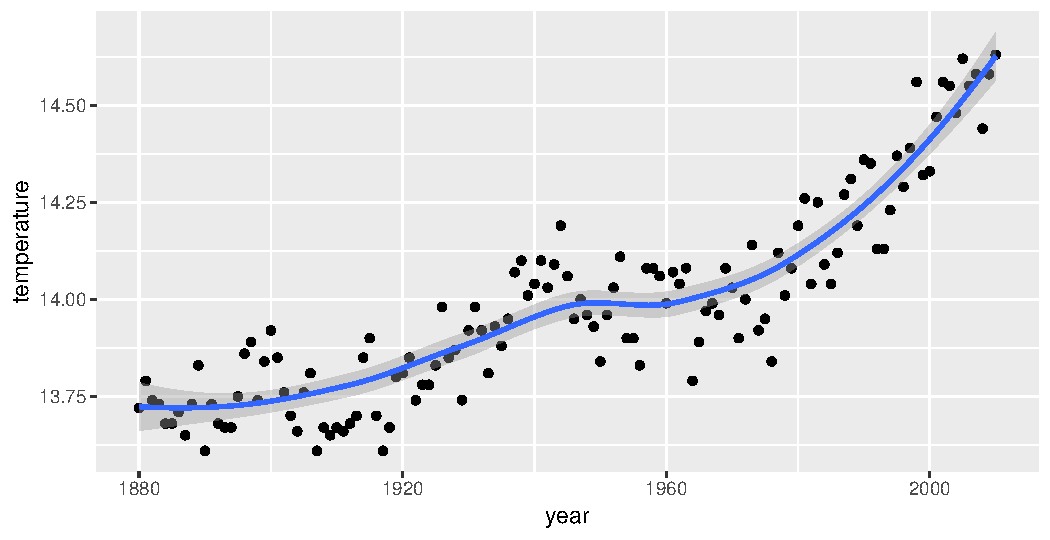
\includegraphics{figure/unnamed-chunk-6-1.pdf}

\end{frame}

\begin{frame}[fragile]{Examining trend}
\protect\hypertarget{examining-trend}{}

\begin{itemize}
\tightlist
\item
  Temperatures increasing on average over time, but pattern very
  irregular.
\item
  Find (Pearson) correlation with time, and test for significance:
\end{itemize}

\begin{Shaded}
\begin{Highlighting}[]
\KeywordTok{with}\NormalTok{(temp, }\KeywordTok{cor.test}\NormalTok{(temperature,year))}
\end{Highlighting}
\end{Shaded}

\begin{verbatim}
## 
##  Pearson's product-moment correlation
## 
## data:  temperature and year
## t = 19.996, df = 129, p-value < 2.2e-16
## alternative hypothesis: true correlation is not equal to 0
## 95 percent confidence interval:
##  0.8203548 0.9059362
## sample estimates:
##       cor 
## 0.8695276
\end{verbatim}

\end{frame}

\begin{frame}{Comments xxx}
\protect\hypertarget{comments-xxx}{}

\begin{itemize}
\tightlist
\item
  Correlation, 0.8695, significantly different from zero.
\item
  CI shows how far from zero it is.
\end{itemize}

Tests for \emph{linear} trend with \emph{normal} data.

\end{frame}

\begin{frame}[fragile]{Kendall correlation}
\protect\hypertarget{kendall-correlation}{}

Alternative, Kendall (rank) correlation, which just tests for monotone
trend (anything upward, anything downward) and is resistant to outliers:

\begin{Shaded}
\begin{Highlighting}[]
\KeywordTok{with}\NormalTok{(temp, }\KeywordTok{cor.test}\NormalTok{(temperature,year,}\DataTypeTok{method=}\StringTok{"kendall"}\NormalTok{))}
\end{Highlighting}
\end{Shaded}

\begin{verbatim}
## 
##  Kendall's rank correlation tau
## 
## data:  temperature and year
## z = 11.776, p-value < 2.2e-16
## alternative hypothesis: true tau is not equal to 0
## sample estimates:
##       tau 
## 0.6992574
\end{verbatim}

Kendall correlation usually closer to 0 for same data, but here P-values
comparable. Trend again strongly significant.

\end{frame}

\begin{frame}[fragile]{Mann-Kendall}
\protect\hypertarget{mann-kendall}{}

\begin{itemize}
\item
  Another way is via \textbf{Mann-Kendall}: Kendall correlation with
  time.
\item
  Use my package \texttt{mkac}:
\end{itemize}

\footnotesize

\begin{Shaded}
\begin{Highlighting}[]
\KeywordTok{kendall_Z_adjusted}\NormalTok{(temp}\OperatorTok{$}\NormalTok{temperature)}
\end{Highlighting}
\end{Shaded}

\begin{verbatim}
## $z
## [1] 11.77267
## 
## $z_star
## [1] 4.475666
## 
## $ratio
## [1] 6.918858
## 
## $P_value
## [1] 0
## 
## $P_value_adj
## [1] 7.617357e-06
\end{verbatim}

\normalsize

\end{frame}

\begin{frame}{Comments}
\protect\hypertarget{comments}{}

P-value is very small, but adjusted one not as small as before because
of \emph{autocorrelation} (see later). Idea: observations close together
in time are correlated with each other, so observations not independent.
This is correction for that.

\end{frame}

\begin{frame}{Examining rate of change}
\protect\hypertarget{examining-rate-of-change}{}

\begin{itemize}
\item
  Having seen that there \emph{is} a change, question is ``how fast is
  it?''
\item
  Examine slopes:

  \begin{itemize}
  \tightlist
  \item
    regular regression slope, if you believe straight-line regression
  \item
    Theil-Sen slope: resistant to outliers, based on medians
  \end{itemize}
\end{itemize}

\end{frame}

\begin{frame}[fragile]{Ordinary regression against time xxx}
\protect\hypertarget{ordinary-regression-against-time-xxx}{}

\begin{Shaded}
\begin{Highlighting}[]
\NormalTok{temp.lm=}\KeywordTok{lm}\NormalTok{(temperature}\OperatorTok{~}\NormalTok{year, }\DataTypeTok{data=}\NormalTok{temp)}
\KeywordTok{summary}\NormalTok{(temp.lm)}
\end{Highlighting}
\end{Shaded}

\begin{verbatim}
## 
## Call:
## lm(formula = temperature ~ year, data = temp)
## 
## Residuals:
##      Min       1Q   Median       3Q      Max 
## -0.32496 -0.10117  0.00575  0.08355  0.28501 
## 
## Coefficients:
##              Estimate Std. Error t value Pr(>|t|)
## (Intercept) 2.5794197  0.5703984   4.522 1.37e-05
## year        0.0058631  0.0002932  19.996  < 2e-16
##                
## (Intercept) ***
## year        ***
## ---
## Signif. codes:  
## 0 '***' 0.001 '**' 0.01 '*' 0.05 '.' 0.1 ' ' 1
## 
## Residual standard error: 0.1269 on 129 degrees of freedom
## Multiple R-squared:  0.7561, Adjusted R-squared:  0.7542 
## F-statistic: 399.9 on 1 and 129 DF,  p-value: < 2.2e-16
\end{verbatim}

Slope about 0.006 degrees per year (about this many degrees over course
of data):

\begin{Shaded}
\begin{Highlighting}[]
\KeywordTok{coef}\NormalTok{(temp.lm)[}\DecValTok{2}\NormalTok{]}\OperatorTok{*}\DecValTok{130}
\end{Highlighting}
\end{Shaded}

\begin{verbatim}
##      year 
## 0.7622068
\end{verbatim}

\end{frame}

\begin{frame}[fragile]{Theil-Sen slope}
\protect\hypertarget{theil-sen-slope}{}

also from \texttt{mkac}:

\begin{Shaded}
\begin{Highlighting}[]
\KeywordTok{theil_sen_slope}\NormalTok{(temp}\OperatorTok{$}\NormalTok{temperature)}
\end{Highlighting}
\end{Shaded}

\begin{verbatim}
## [1] 0.005675676
\end{verbatim}

\end{frame}

\begin{frame}{Conclusions}
\protect\hypertarget{conclusions}{}

\begin{itemize}
\tightlist
\item
  Slopes:

  \begin{itemize}
  \tightlist
  \item
    Linear regression: 0.005863
  \item
    Theil-Sen slope: 0.005676
  \item
    Very close.
  \end{itemize}
\item
  Correlations:

  \begin{itemize}
  \tightlist
  \item
    Pearson 0.8675
  \item
    Kendall 0.6993
  \item
    Kendall correlation smaller, but P-value equally significant (often
    the case)
  \end{itemize}
\end{itemize}

\end{frame}

\begin{frame}[fragile]{Constant rate of change? xxx}
\protect\hypertarget{constant-rate-of-change-xxx}{}

Slope assumes that the rate of change is same over all years, but trend
seemed to be accelerating: xxx

\begin{Shaded}
\begin{Highlighting}[]
\KeywordTok{ggplot}\NormalTok{(temp, }\KeywordTok{aes}\NormalTok{(}\DataTypeTok{x=}\NormalTok{year, }\DataTypeTok{y=}\NormalTok{temperature)) }\OperatorTok{+}\StringTok{ }
\StringTok{  }\KeywordTok{geom_point}\NormalTok{() }\OperatorTok{+}\StringTok{ }\KeywordTok{geom_smooth}\NormalTok{()}
\end{Highlighting}
\end{Shaded}

\begin{verbatim}
## `geom_smooth()` using method = 'loess' and formula 'y ~ x'
\end{verbatim}

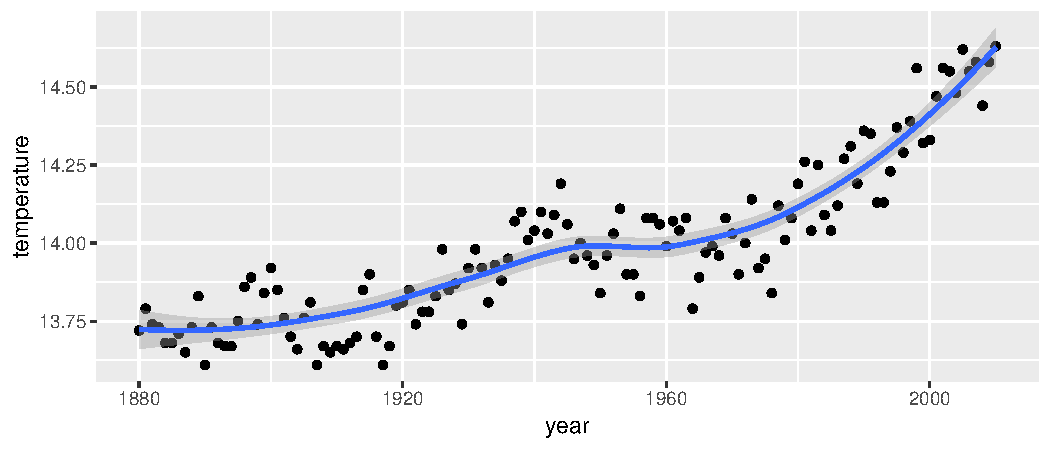
\includegraphics{figure/unnamed-chunk-13-1.pdf}

\end{frame}

\begin{frame}[fragile]{Pre-1970 and post-1970: xxx}
\protect\hypertarget{pre-1970-and-post-1970-xxx}{}

\begin{Shaded}
\begin{Highlighting}[]
\NormalTok{temp }\OperatorTok\StringTok{ }
\StringTok{  }\KeywordTok{mutate}\NormalTok{(}\DataTypeTok{time_period=}\KeywordTok{ifelse}\NormalTok{(year}\OperatorTok{<=}\DecValTok{1970}\NormalTok{, }\StringTok{"pre-1970"}\NormalTok{, }\StringTok{"post-1970"}\NormalTok{)) }\OperatorTok\StringTok{ }
\StringTok{  }\KeywordTok{nest}\NormalTok{(}\OperatorTok{-}\NormalTok{time_period) }\OperatorTok\StringTok{ }
\StringTok{  }\KeywordTok{mutate}\NormalTok{(}\DataTypeTok{theil_sen=}\KeywordTok{map_dbl}\NormalTok{(}
\NormalTok{    data, }\OperatorTok{~}\KeywordTok{theil_sen_slope}\NormalTok{(.}\OperatorTok{$}\NormalTok{temperature)))}
\end{Highlighting}
\end{Shaded}

\begin{verbatim}
## # A tibble: 2 x 3
##   time_period data              theil_sen
##   <chr>       <list>                <dbl>
## 1 pre-1970    <tibble [91 × 4]>   0.00429
## 2 post-1970   <tibble [40 × 4]>   0.0168
\end{verbatim}

Theil-Sen slope is very nearly \emph{four times} as big since 1970
vs.~before.

\end{frame}

\begin{frame}[fragile]{Actual time series: the Kings of England}
\protect\hypertarget{actual-time-series-the-kings-of-england}{}

\begin{itemize}
\tightlist
\item
  Age at death of Kings and Queens of England since William the
  Conqueror (1066):
\end{itemize}

\begin{Shaded}
\begin{Highlighting}[]
\NormalTok{kings=}\KeywordTok{read_table}\NormalTok{(}\StringTok{"kings.txt"}\NormalTok{, }\DataTypeTok{col_names=}\NormalTok{F)}
\end{Highlighting}
\end{Shaded}

\begin{verbatim}
## Parsed with column specification:
## cols(
##   X1 = col_double()
## )
\end{verbatim}

Data in one long column \texttt{X1}, so \texttt{kings} is data frame
with one column.

\end{frame}

\begin{frame}[fragile]{Turn into \texttt{ts} time series object}
\protect\hypertarget{turn-into-ts-time-series-object}{}

\begin{Shaded}
\begin{Highlighting}[]
\NormalTok{kings.ts=}\KeywordTok{ts}\NormalTok{(kings)}
\NormalTok{kings.ts}
\end{Highlighting}
\end{Shaded}

\begin{verbatim}
## Time Series:
## Start = 1 
## End = 42 
## Frequency = 1 
##       X1
##  [1,] 60
##  [2,] 43
##  [3,] 67
##  [4,] 50
##  [5,] 56
##  [6,] 42
##  [7,] 50
##  [8,] 65
##  [9,] 68
## [10,] 43
## [11,] 65
## [12,] 34
## [13,] 47
## [14,] 34
## [15,] 49
## [16,] 41
## [17,] 13
## [18,] 35
## [19,] 53
## [20,] 56
## [21,] 16
## [22,] 43
## [23,] 69
## [24,] 59
## [25,] 48
## [26,] 59
## [27,] 86
## [28,] 55
## [29,] 68
## [30,] 51
## [31,] 33
## [32,] 49
## [33,] 67
## [34,] 77
## [35,] 81
## [36,] 67
## [37,] 71
## [38,] 81
## [39,] 68
## [40,] 70
## [41,] 77
## [42,] 56
\end{verbatim}

\end{frame}

\begin{frame}[fragile]{Plotting a time series}
\protect\hypertarget{plotting-a-time-series}{}

\texttt{autoplot} from \texttt{ggfortify} gives time plot:

\begin{Shaded}
\begin{Highlighting}[]
\KeywordTok{autoplot}\NormalTok{(kings.ts)}
\end{Highlighting}
\end{Shaded}

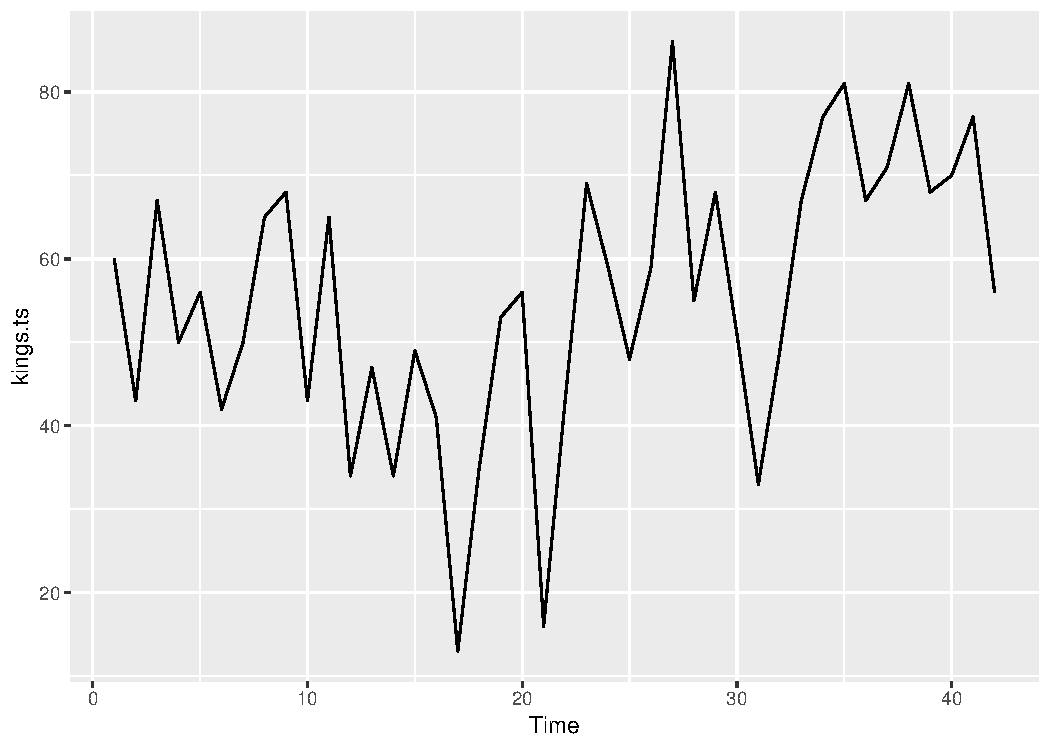
\includegraphics{figure/Kings-Time-Series-1.pdf}

\end{frame}

\begin{frame}{Comments}
\protect\hypertarget{comments-1}{}

\begin{itemize}
\item
  ``Time'' here is order of monarch from William the Conqueror (1st) to
  George VI (last).
\item
  Looks to be slightly increasing trend of age-at-death
\item
  but lots of irregularity.
\end{itemize}

\end{frame}

\begin{frame}{Stationarity}
\protect\hypertarget{stationarity}{}

A time series is \textbf{stationary} if:

\begin{itemize}
\tightlist
\item
  mean is constant over time
\item
  variability constant over time and not changing with mean.
\end{itemize}

Kings time series seems to have:

\begin{itemize}
\tightlist
\item
  non-constant mean
\item
  but constant variability
\item
  not stationary.
\end{itemize}

\end{frame}

\begin{frame}[fragile]{Getting it stationary}
\protect\hypertarget{getting-it-stationary}{}

\begin{itemize}
\tightlist
\item
  Usual fix for non-stationarity is \emph{differencing}: new series 2nd
  - 1st, 3rd - 2nd etc.
\end{itemize}

In R, \texttt{diff}:

\begin{Shaded}
\begin{Highlighting}[]
\NormalTok{kings.diff.ts=}\KeywordTok{diff}\NormalTok{(kings.ts)}
\end{Highlighting}
\end{Shaded}

\end{frame}

\begin{frame}[fragile]{Did differencing fix stationarity?}
\protect\hypertarget{did-differencing-fix-stationarity}{}

Looks stationary now: xxx

\begin{Shaded}
\begin{Highlighting}[]
\KeywordTok{autoplot}\NormalTok{(kings.diff.ts)}
\end{Highlighting}
\end{Shaded}

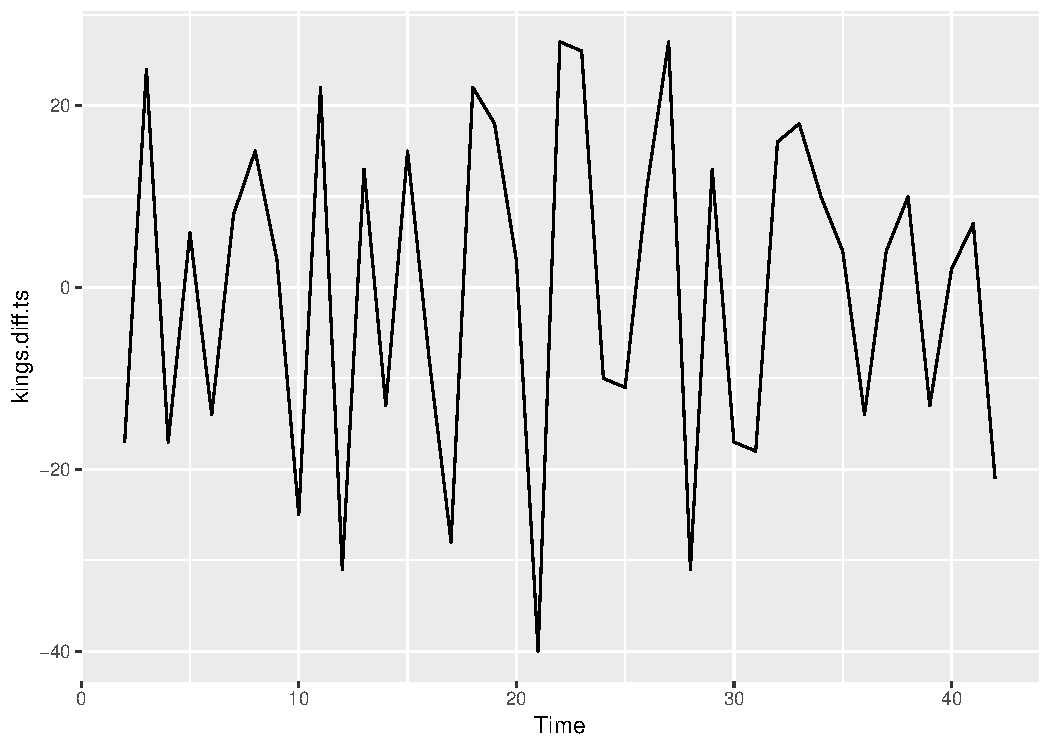
\includegraphics{figure/Differenced-Kings-Series-1.pdf}

\end{frame}

\begin{frame}[fragile]{Births per month in New York City}
\protect\hypertarget{births-per-month-in-new-york-city}{}

from January 1946 to December 1959:

\begin{Shaded}
\begin{Highlighting}[]
\NormalTok{ny=}\KeywordTok{read_table}\NormalTok{(}\StringTok{"nybirths.txt"}\NormalTok{,}\DataTypeTok{col_names=}\NormalTok{F)}
\end{Highlighting}
\end{Shaded}

\begin{verbatim}
## Parsed with column specification:
## cols(
##   X1 = col_double()
## )
\end{verbatim}

\begin{Shaded}
\begin{Highlighting}[]
\NormalTok{ny}
\end{Highlighting}
\end{Shaded}

\begin{verbatim}
## # A tibble: 168 x 1
##       X1
##    <dbl>
##  1  26.7
##  2  23.6
##  3  26.9
##  4  24.7
##  5  25.8
##  6  24.4
##  7  24.5
##  8  23.9
##  9  23.2
## 10  23.2
## # … with 158 more rows
\end{verbatim}

\begin{Shaded}
\begin{Highlighting}[]
\NormalTok{ny.ts=}\KeywordTok{ts}\NormalTok{(ny,}\DataTypeTok{freq=}\DecValTok{12}\NormalTok{,}\DataTypeTok{start=}\KeywordTok{c}\NormalTok{(}\DecValTok{1946}\NormalTok{,}\DecValTok{1}\NormalTok{))}
\NormalTok{ny.ts}
\end{Highlighting}
\end{Shaded}

\begin{verbatim}
##         Jan    Feb    Mar    Apr    May    Jun
## 1946 26.663 23.598 26.931 24.740 25.806 24.364
## 1947 21.439 21.089 23.709 21.669 21.752 20.761
## 1948 21.937 20.035 23.590 21.672 22.222 22.123
## 1949 21.548 20.000 22.424 20.615 21.761 22.874
## 1950 22.604 20.894 24.677 23.673 25.320 23.583
## 1951 23.287 23.049 25.076 24.037 24.430 24.667
## 1952 23.798 22.270 24.775 22.646 23.988 24.737
## 1953 24.364 22.644 25.565 24.062 25.431 24.635
## 1954 24.657 23.304 26.982 26.199 27.210 26.122
## 1955 24.990 24.239 26.721 23.475 24.767 26.219
## 1956 26.217 24.218 27.914 26.975 28.527 27.139
## 1957 26.589 24.848 27.543 26.896 28.878 27.390
## 1958 27.132 24.924 28.963 26.589 27.931 28.009
## 1959 26.076 25.286 27.660 25.951 26.398 25.565
##         Jul    Aug    Sep    Oct    Nov    Dec
## 1946 24.477 23.901 23.175 23.227 21.672 21.870
## 1947 23.479 23.824 23.105 23.110 21.759 22.073
## 1948 23.950 23.504 22.238 23.142 21.059 21.573
## 1949 24.104 23.748 23.262 22.907 21.519 22.025
## 1950 24.671 24.454 24.122 24.252 22.084 22.991
## 1951 26.451 25.618 25.014 25.110 22.964 23.981
## 1952 26.276 25.816 25.210 25.199 23.162 24.707
## 1953 27.009 26.606 26.268 26.462 25.246 25.180
## 1954 26.706 26.878 26.152 26.379 24.712 25.688
## 1955 28.361 28.599 27.914 27.784 25.693 26.881
## 1956 28.982 28.169 28.056 29.136 26.291 26.987
## 1957 28.065 28.141 29.048 28.484 26.634 27.735
## 1958 29.229 28.759 28.405 27.945 25.912 26.619
## 1959 28.865 30.000 29.261 29.012 26.992 27.897
\end{verbatim}

Note extras on \texttt{ts}:

\begin{itemize}
\tightlist
\item
  Time period is 1 year
\item
  12 observations per year (monthly) in \texttt{freq}
\item
  First observation is 1st month of 1946 in \texttt{start} xxx more
\end{itemize}

Printing formats nicely.

\end{frame}

\begin{frame}[fragile]{Time plot}
\protect\hypertarget{time-plot}{}

\begin{itemize}
\tightlist
\item
  Time plot shows extra pattern: xxx
\end{itemize}

\begin{Shaded}
\begin{Highlighting}[]
\KeywordTok{autoplot}\NormalTok{(ny.ts)}
\end{Highlighting}
\end{Shaded}

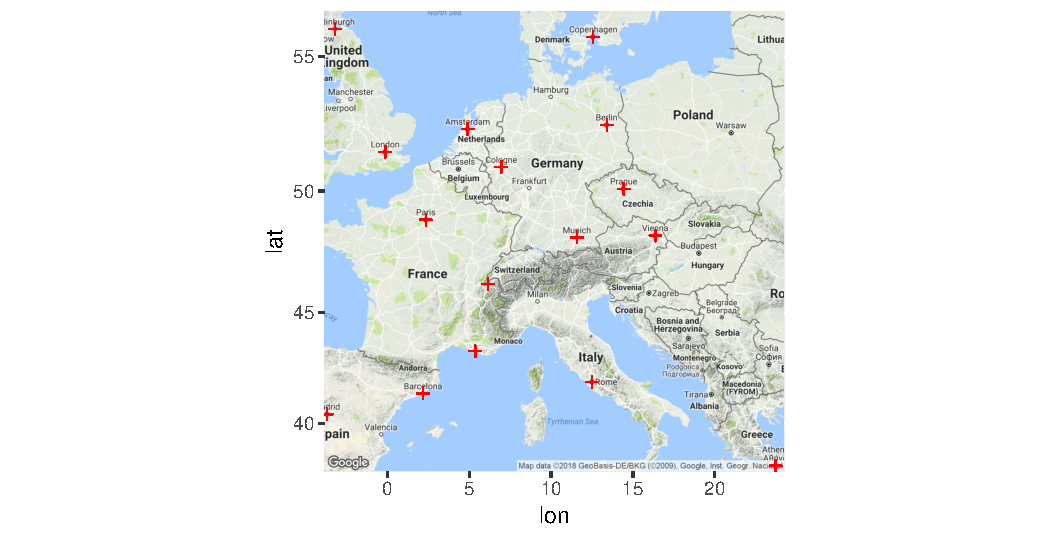
\includegraphics{figure/unnamed-chunk-19-1.pdf}

\end{frame}

\begin{frame}{Comments on time plot}
\protect\hypertarget{comments-on-time-plot}{}

\begin{itemize}
\tightlist
\item
  steady increase (after initial drop)
\item
  repeating pattern each year (seasonal component).
\item
  Not stationary.
\end{itemize}

\end{frame}

\begin{frame}[fragile]{Differencing the New York births}
\protect\hypertarget{differencing-the-new-york-births}{}

Does differencing help here? xxx

\begin{Shaded}
\begin{Highlighting}[]
\NormalTok{ny.diff.ts=}\KeywordTok{diff}\NormalTok{(ny.ts)}
\KeywordTok{autoplot}\NormalTok{(ny.diff.ts)}
\end{Highlighting}
\end{Shaded}

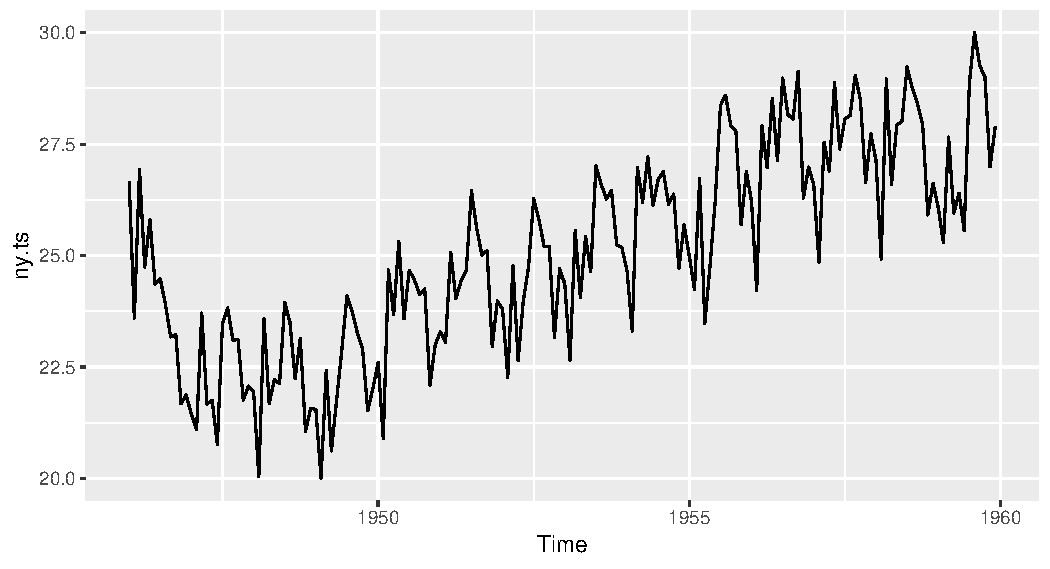
\includegraphics{figure/unnamed-chunk-20-1.pdf}

Looks stationary, but some regular spikes.

\end{frame}

\begin{frame}[fragile]{Decomposing a seasonal time series}
\protect\hypertarget{decomposing-a-seasonal-time-series}{}

Observations for NY births were every month. Are things the same every
year?

A visual (using original data): xxx

\begin{Shaded}
\begin{Highlighting}[]
\KeywordTok{decompose}\NormalTok{(ny.ts) }\OperatorTok\StringTok{ }\KeywordTok{autoplot}\NormalTok{()}
\end{Highlighting}
\end{Shaded}

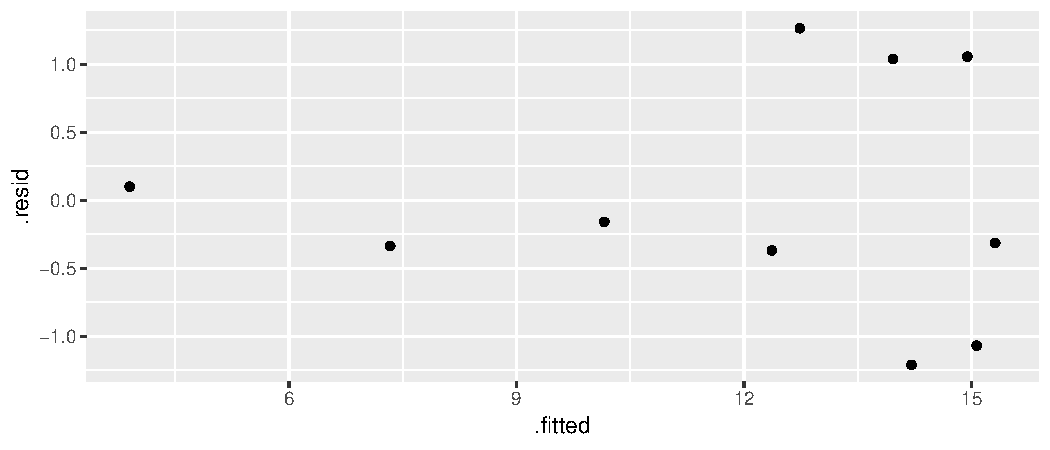
\includegraphics{figure/unnamed-chunk-21-1.pdf}

\end{frame}

\begin{frame}{Decomposition bits}
\protect\hypertarget{decomposition-bits}{}

Shows:

\begin{itemize}
\tightlist
\item
  original series
\item
  a ``seasonal'' part: something that repeats every year
\item
  just the trend, going steadily up (except at the start)
\item
  random: what is left over (``remainder'')
\end{itemize}

\end{frame}

\begin{frame}[fragile]{The seasonal part}
\protect\hypertarget{the-seasonal-part}{}

Fitted seasonal part is same every year, births lowest in February and
highest in July:

\begin{Shaded}
\begin{Highlighting}[]
\NormalTok{ny.d}\OperatorTok{$}\NormalTok{seasonal}
\end{Highlighting}
\end{Shaded}

\begin{verbatim}
## Error in eval(expr, envir, enclos): object 'ny.d' not found
\end{verbatim}

\end{frame}

\begin{frame}{Time series basics}
\protect\hypertarget{time-series-basics}{}

\end{frame}

\begin{frame}[fragile]{White noise}
\protect\hypertarget{white-noise}{}

Independent random normal. Knowing one value tells you nothing about the
next. ``Random'' process. xxx

\begin{Shaded}
\begin{Highlighting}[]
\NormalTok{wn=}\KeywordTok{rnorm}\NormalTok{(}\DecValTok{100}\NormalTok{)}
\NormalTok{wn.ts=}\KeywordTok{ts}\NormalTok{(wn)}
\KeywordTok{autoplot}\NormalTok{(wn.ts)}
\end{Highlighting}
\end{Shaded}

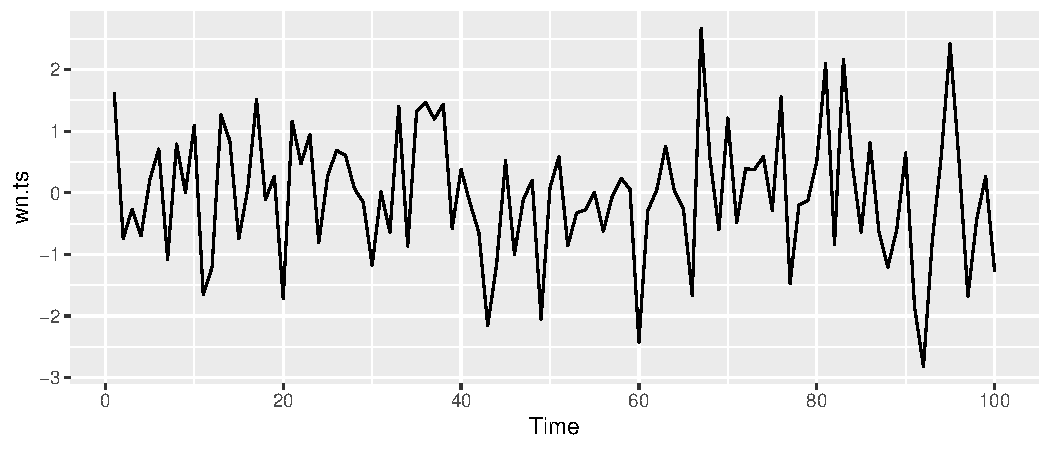
\includegraphics{figure/White-Noise-1.pdf}

\end{frame}

\begin{frame}[fragile]{Lagging a time series}
\protect\hypertarget{lagging-a-time-series}{}

This means moving a time series one (or more) steps back in time:

\begin{Shaded}
\begin{Highlighting}[]
\NormalTok{x=}\KeywordTok{rnorm}\NormalTok{(}\DecValTok{5}\NormalTok{)}
\KeywordTok{tibble}\NormalTok{(x) }\OperatorTok\StringTok{ }\KeywordTok{mutate}\NormalTok{(}\DataTypeTok{x_lagged=}\KeywordTok{lag}\NormalTok{(x)) ->}\StringTok{ }\NormalTok{with_lagged}
\NormalTok{with_lagged}
\end{Highlighting}
\end{Shaded}

\begin{verbatim}
## # A tibble: 5 x 2
##         x x_lagged
##     <dbl>    <dbl>
## 1 -2.04     NA    
## 2 -0.579    -2.04 
## 3  0.608    -0.579
## 4  0.118     0.608
## 5  0.0563    0.118
\end{verbatim}

Gain a missing because there is nothing before the first observation.

\end{frame}

\begin{frame}[fragile]{Lagging white noise}
\protect\hypertarget{lagging-white-noise}{}

\begin{Shaded}
\begin{Highlighting}[]
\KeywordTok{tibble}\NormalTok{(wn) }\OperatorTok\StringTok{ }\KeywordTok{mutate}\NormalTok{(}\DataTypeTok{wn_lagged=}\KeywordTok{lag}\NormalTok{(wn)) ->}\StringTok{ }\NormalTok{wn_with_lagged}
\KeywordTok{ggplot}\NormalTok{(wn_with_lagged, }\KeywordTok{aes}\NormalTok{(}\DataTypeTok{y=}\NormalTok{wn, }\DataTypeTok{x=}\NormalTok{wn_lagged))}\OperatorTok{+}\KeywordTok{geom_point}\NormalTok{()}
\end{Highlighting}
\end{Shaded}

\begin{verbatim}
## Warning: Removed 1 rows containing missing values
## (geom_point).
\end{verbatim}

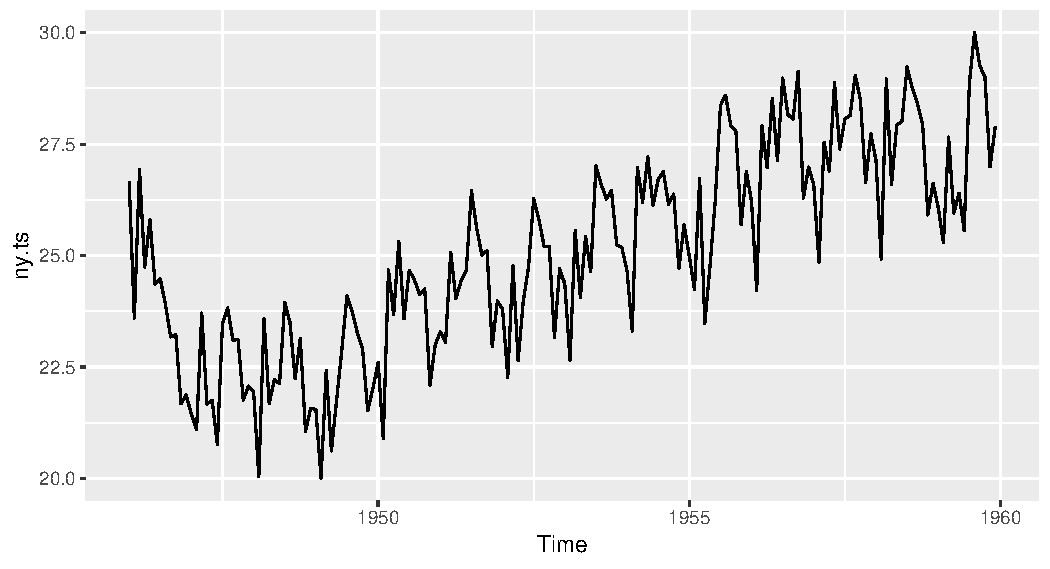
\includegraphics{figure/unnamed-chunk-25-1.pdf}

\begin{Shaded}
\begin{Highlighting}[]
\KeywordTok{with}\NormalTok{(wn_with_lagged, }\KeywordTok{cor.test}\NormalTok{(wn, wn_lagged, }\DataTypeTok{use=}\StringTok{"c"}\NormalTok{)) }\CommentTok{# ignore the missing value}
\end{Highlighting}
\end{Shaded}

\begin{verbatim}
## 
##  Pearson's product-moment correlation
## 
## data:  wn and wn_lagged
## t = -0.16512, df = 97, p-value = 0.8692
## alternative hypothesis: true correlation is not equal to 0
## 95 percent confidence interval:
##  -0.213468  0.181249
## sample estimates:
##         cor 
## -0.01676257
\end{verbatim}

\end{frame}

\begin{frame}[fragile]{Correlation with lagged series}
\protect\hypertarget{correlation-with-lagged-series}{}

If you know about white noise at one time point, you know \emph{nothing}
about it at the next. This is shown by the scatterplot and the
correlation.

On the other hand, this:

\begin{Shaded}
\begin{Highlighting}[]
\KeywordTok{tibble}\NormalTok{(}\DataTypeTok{age=}\NormalTok{kings}\OperatorTok{$}\NormalTok{X1) }\OperatorTok\StringTok{ }
\StringTok{  }\KeywordTok{mutate}\NormalTok{(}\DataTypeTok{age_lagged=}\KeywordTok{lag}\NormalTok{(age)) ->}\StringTok{ }\NormalTok{kings_with_lagged}
\KeywordTok{with}\NormalTok{(kings_with_lagged, }\KeywordTok{cor.test}\NormalTok{(age, age_lagged))}
\end{Highlighting}
\end{Shaded}

\begin{verbatim}
## 
##  Pearson's product-moment correlation
## 
## data:  age and age_lagged
## t = 2.7336, df = 39, p-value = 0.00937
## alternative hypothesis: true correlation is not equal to 0
## 95 percent confidence interval:
##  0.1064770 0.6308209
## sample estimates:
##       cor 
## 0.4009919
\end{verbatim}

\end{frame}

\begin{frame}[fragile]{If one value larger, the next value (a bit) more
likely to be larger:}
\protect\hypertarget{if-one-value-larger-the-next-value-a-bit-more-likely-to-be-larger}{}

\begin{Shaded}
\begin{Highlighting}[]
\KeywordTok{ggplot}\NormalTok{(kings_with_lagged, }\KeywordTok{aes}\NormalTok{(}\DataTypeTok{x=}\NormalTok{age_lagged, }\DataTypeTok{y=}\NormalTok{age)) }\OperatorTok{+}\StringTok{ }\KeywordTok{geom_point}\NormalTok{()}
\end{Highlighting}
\end{Shaded}

\begin{verbatim}
## Warning: Removed 1 rows containing missing values
## (geom_point).
\end{verbatim}

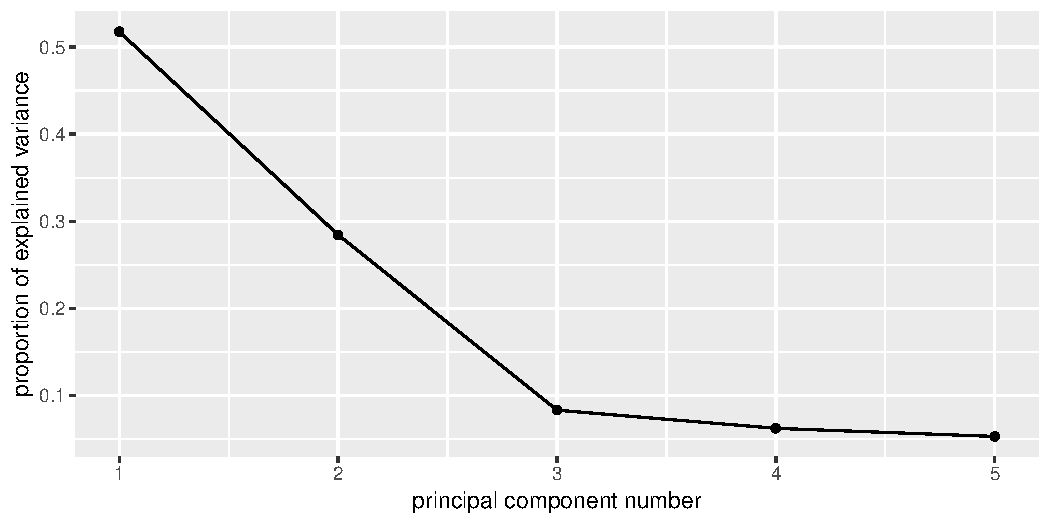
\includegraphics{figure/unnamed-chunk-27-1.pdf}

\end{frame}

\begin{frame}[fragile]{Two steps back:}
\protect\hypertarget{two-steps-back}{}

\begin{Shaded}
\begin{Highlighting}[]
\NormalTok{kings_with_lagged }\OperatorTok\StringTok{ }
\StringTok{  }\KeywordTok{mutate}\NormalTok{(}\DataTypeTok{age_lag_2=}\KeywordTok{lag}\NormalTok{(age_lagged)) }\OperatorTok\StringTok{ }
\StringTok{  }\KeywordTok{with}\NormalTok{(., }\KeywordTok{cor.test}\NormalTok{(age, age_lag_}\DecValTok{2}\NormalTok{))}
\end{Highlighting}
\end{Shaded}

\begin{verbatim}
## 
##  Pearson's product-moment correlation
## 
## data:  age and age_lag_2
## t = 1.5623, df = 38, p-value = 0.1265
## alternative hypothesis: true correlation is not equal to 0
## 95 percent confidence interval:
##  -0.07128917  0.51757510
## sample estimates:
##      cor 
## 0.245676
\end{verbatim}

Still a correlation two steps back, but smaller (and no longer
significant).

\end{frame}

\begin{frame}[fragile]{Autocorrelation}
\protect\hypertarget{autocorrelation}{}

Correlation of time series with \emph{itself} one, two,\ldots{} time
steps back is useful idea, called \textbf{autocorrelation}. Make a plot
of it with \texttt{acf} and \texttt{autoplot}:

White noise: xxx

\begin{Shaded}
\begin{Highlighting}[]
\KeywordTok{acf}\NormalTok{(wn.ts, }\DataTypeTok{plot=}\NormalTok{F) }\OperatorTok\StringTok{ }\KeywordTok{autoplot}\NormalTok{()}
\end{Highlighting}
\end{Shaded}

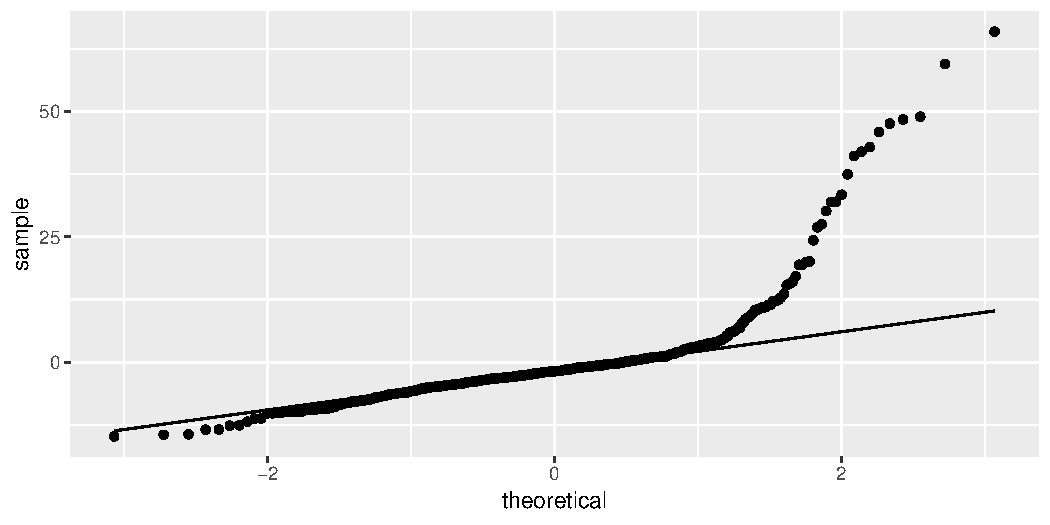
\includegraphics{figure/unnamed-chunk-29-1.pdf}

No autocorrelations beyond chance, anywhere (except \emph{possibly} at
lag 13).

Autocorrelations work best on \emph{stationary} series.

\end{frame}

\begin{frame}[fragile]{Kings, differenced xxx}
\protect\hypertarget{kings-differenced-xxx}{}

\begin{Shaded}
\begin{Highlighting}[]
\KeywordTok{acf}\NormalTok{(kings.diff.ts, }\DataTypeTok{plot=}\NormalTok{F) }\OperatorTok\StringTok{ }\KeywordTok{autoplot}\NormalTok{()}
\end{Highlighting}
\end{Shaded}

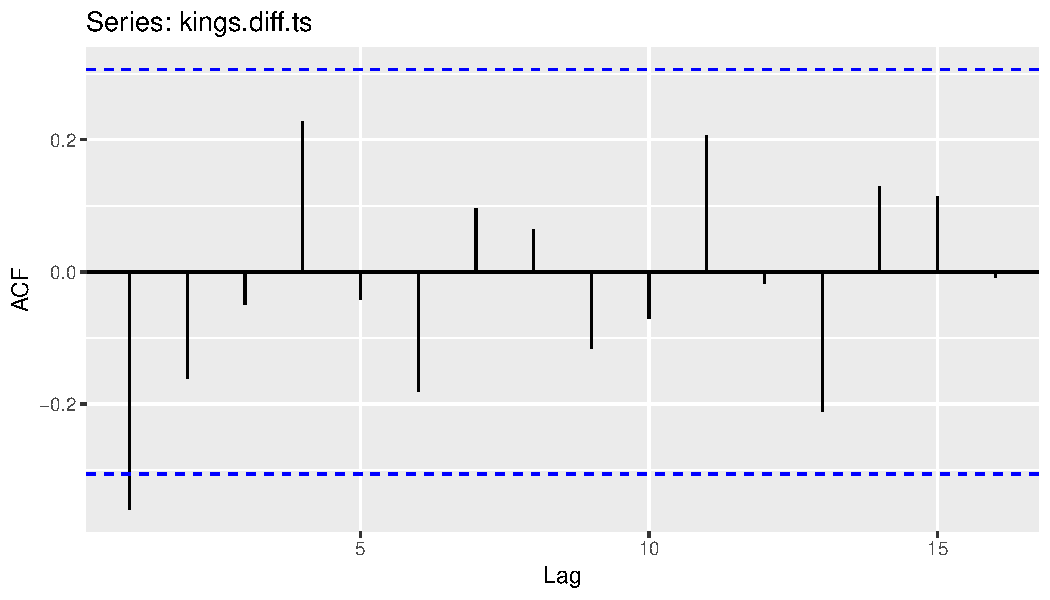
\includegraphics{figure/unnamed-chunk-30-1.pdf}

\end{frame}

\begin{frame}{Comments on autocorrelations of kings series}
\protect\hypertarget{comments-on-autocorrelations-of-kings-series}{}

Negative autocorrelation at lag 1, nothing beyond that.

\begin{itemize}
\tightlist
\item
  If one value of differenced series positive, next one most likely
  negative.
\item
  If one king lives longer than predecessor, next one likely lives
  shorter.
\end{itemize}

\end{frame}

\begin{frame}[fragile]{NY births, differenced xxx}
\protect\hypertarget{ny-births-differenced-xxx}{}

\begin{Shaded}
\begin{Highlighting}[]
\KeywordTok{acf}\NormalTok{(ny.diff.ts, }\DataTypeTok{plot=}\NormalTok{F) }\OperatorTok\StringTok{ }\KeywordTok{autoplot}\NormalTok{()}
\end{Highlighting}
\end{Shaded}

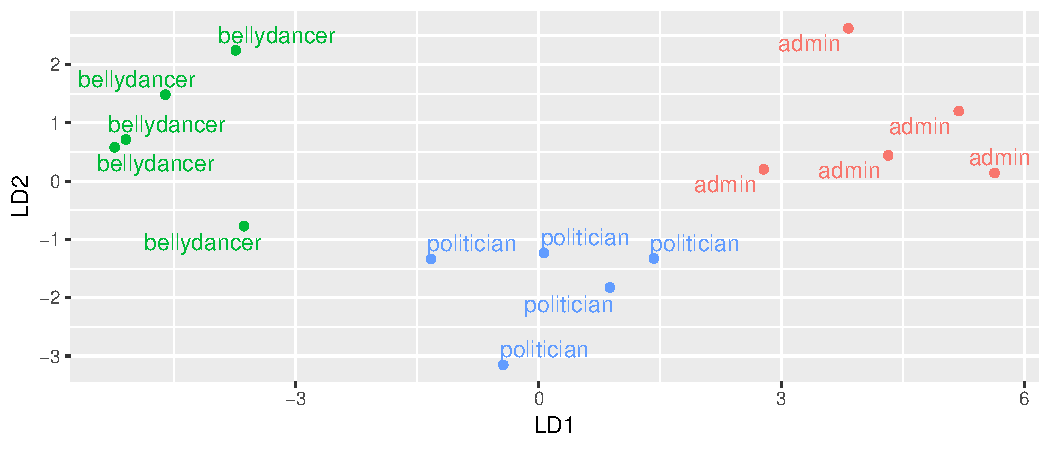
\includegraphics{figure/unnamed-chunk-31-1.pdf}

\end{frame}

\begin{frame}{Lots of stuff:}
\protect\hypertarget{lots-of-stuff}{}

\begin{itemize}
\tightlist
\item
  large positive autocorrelation at 1.0 years (July one year like July
  last year)
\item
  large negative autocorrelation at 1 month.
\item
  smallish but significant negative autocorrelation at 0.5 year = 6
  months.
\item
  Other stuff -- complicated.
\end{itemize}

\end{frame}

\begin{frame}[fragile]{Souvenir sales}
\protect\hypertarget{souvenir-sales}{}

Monthly sales for a beach souvenir shop in Queensland, Australia:

\begin{Shaded}
\begin{Highlighting}[]
\NormalTok{souv=}\KeywordTok{read_table}\NormalTok{(}\StringTok{"souvenir.txt"}\NormalTok{, }\DataTypeTok{col_names=}\NormalTok{F)}
\end{Highlighting}
\end{Shaded}

\begin{verbatim}
## Parsed with column specification:
## cols(
##   X1 = col_double()
## )
\end{verbatim}

\begin{Shaded}
\begin{Highlighting}[]
\NormalTok{souv.ts=}\KeywordTok{ts}\NormalTok{(souv,}\DataTypeTok{frequency=}\DecValTok{12}\NormalTok{,}\DataTypeTok{start=}\DecValTok{1987}\NormalTok{)}
\NormalTok{souv.ts}
\end{Highlighting}
\end{Shaded}

\begin{verbatim}
##            Jan       Feb       Mar       Apr
## 1987   1664.81   2397.53   2840.71   3547.29
## 1988   2499.81   5198.24   7225.14   4806.03
## 1989   4717.02   5702.63   9957.58   5304.78
## 1990   5921.10   5814.58  12421.25   6369.77
## 1991   4826.64   6470.23   9638.77   8821.17
## 1992   7615.03   9849.69  14558.40  11587.33
## 1993  10243.24  11266.88  21826.84  17357.33
##            May       Jun       Jul       Aug
## 1987   3752.96   3714.74   4349.61   3566.34
## 1988   5900.88   4951.34   6179.12   4752.15
## 1989   6492.43   6630.80   7349.62   8176.62
## 1990   7609.12   7224.75   8121.22   7979.25
## 1991   8722.37  10209.48  11276.55  12552.22
## 1992   9332.56  13082.09  16732.78  19888.61
## 1993  15997.79  18601.53  26155.15  28586.52
##            Sep       Oct       Nov       Dec
## 1987   5021.82   6423.48   7600.60  19756.21
## 1988   5496.43   5835.10  12600.08  28541.72
## 1989   8573.17   9690.50  15151.84  34061.01
## 1990   8093.06   8476.70  17914.66  30114.41
## 1991  11637.39  13606.89  21822.11  45060.69
## 1992  23933.38  25391.35  36024.80  80721.71
## 1993  30505.41  30821.33  46634.38 104660.67
\end{verbatim}

\end{frame}

\begin{frame}[fragile]{Plot of souvenir sales xxx}
\protect\hypertarget{plot-of-souvenir-sales-xxx}{}

\begin{Shaded}
\begin{Highlighting}[]
\KeywordTok{autoplot}\NormalTok{(souv.ts)}
\end{Highlighting}
\end{Shaded}

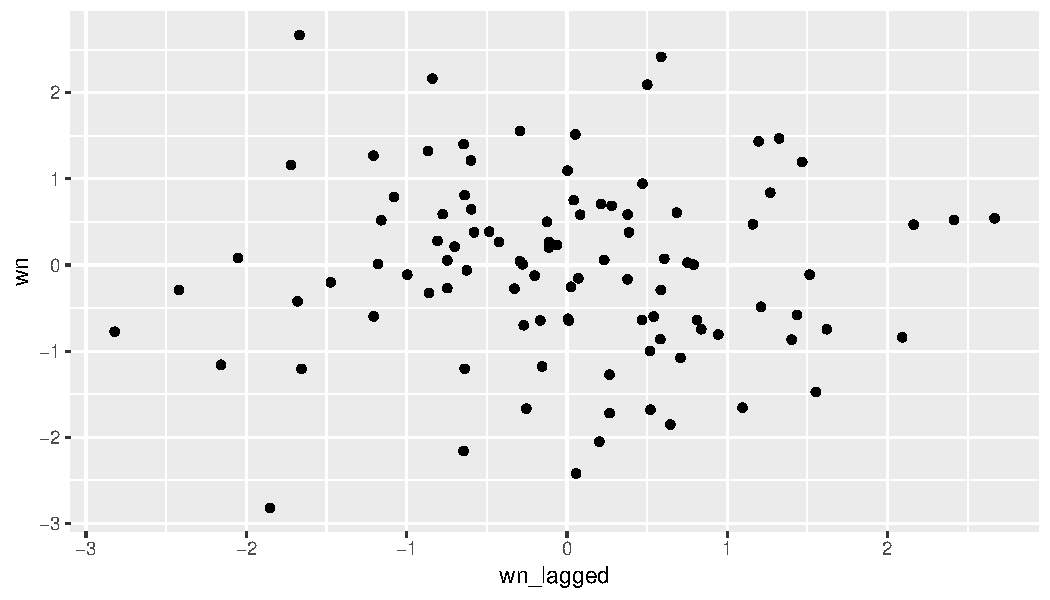
\includegraphics{figure/unnamed-chunk-33-1.pdf}

\end{frame}

\begin{frame}{Several problems:}
\protect\hypertarget{several-problems}{}

\begin{itemize}
\tightlist
\item
  Mean goes up over time
\item
  Variability gets larger as mean gets larger
\item
  Not stationary
\end{itemize}

\end{frame}

\begin{frame}[fragile]{Problem-fixing:}
\protect\hypertarget{problem-fixing}{}

Fix non-constant variability first by taking logs: xxx

\begin{Shaded}
\begin{Highlighting}[]
\NormalTok{souv.log.ts=}\KeywordTok{log}\NormalTok{(souv.ts)}
\KeywordTok{autoplot}\NormalTok{(souv.log.ts)}
\end{Highlighting}
\end{Shaded}

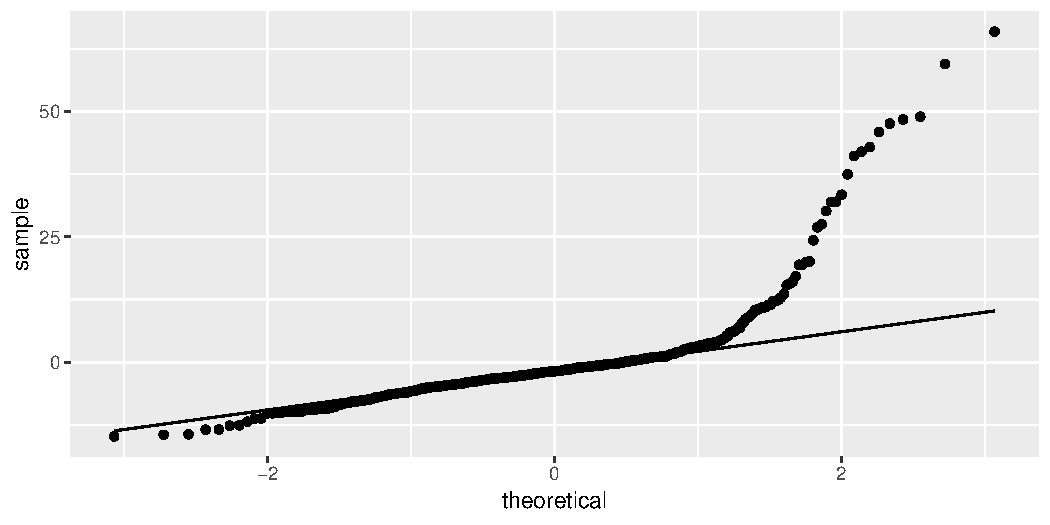
\includegraphics{figure/unnamed-chunk-34-1.pdf}

\end{frame}

\begin{frame}[fragile]{Mean still not constant, so try taking
differences xxx}
\protect\hypertarget{mean-still-not-constant-so-try-taking-differences-xxx}{}

\begin{Shaded}
\begin{Highlighting}[]
\NormalTok{souv.log.diff.ts=}\KeywordTok{diff}\NormalTok{(souv.log.ts)}
\KeywordTok{autoplot}\NormalTok{(souv.log.diff.ts)}
\end{Highlighting}
\end{Shaded}

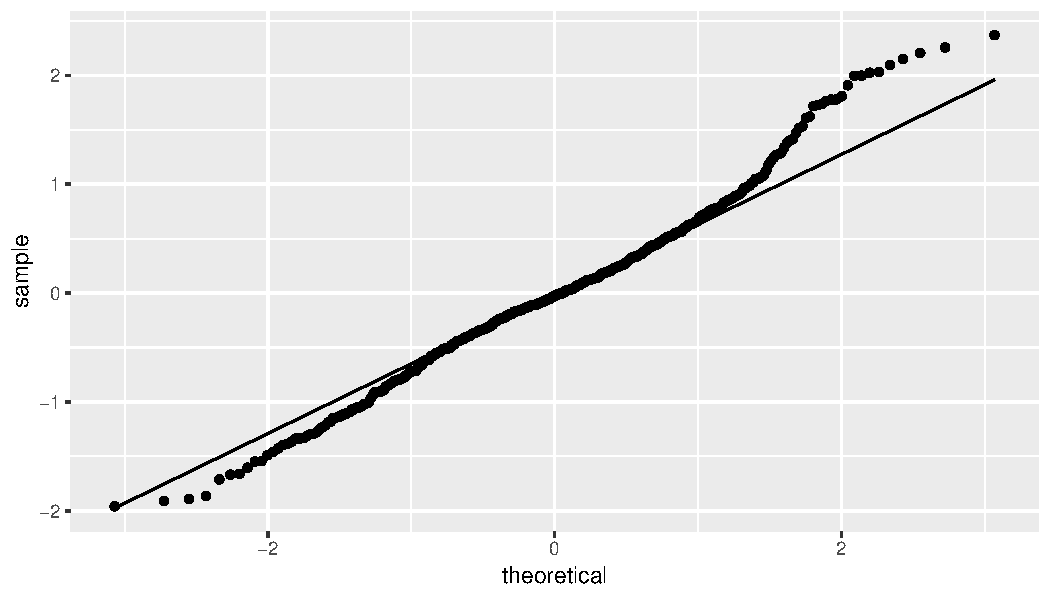
\includegraphics{figure/unnamed-chunk-35-1.pdf}

\end{frame}

\begin{frame}{Comments}
\protect\hypertarget{comments-2}{}

\begin{itemize}
\tightlist
\item
  Now stationary
\item
  but clear seasonal effect.
\end{itemize}

\end{frame}

\begin{frame}[fragile]{Decomposing to see the seasonal effect xxx}
\protect\hypertarget{decomposing-to-see-the-seasonal-effect-xxx}{}

\begin{Shaded}
\begin{Highlighting}[]
\NormalTok{souv.d=}\KeywordTok{decompose}\NormalTok{(souv.log.diff.ts)}
\KeywordTok{autoplot}\NormalTok{(souv.d)}
\end{Highlighting}
\end{Shaded}

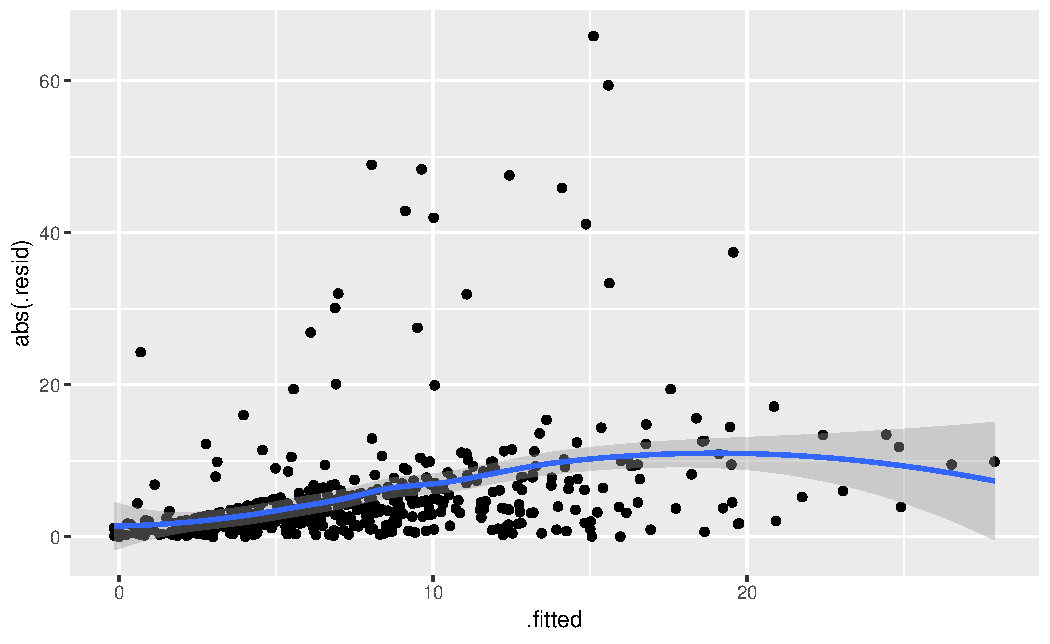
\includegraphics{figure/unnamed-chunk-36-1.pdf}

\end{frame}

\begin{frame}[fragile]{Comments}
\protect\hypertarget{comments-3}{}

\textbf{Big} drop in one month's differences. Look at seasonal component
to see which:

\begin{Shaded}
\begin{Highlighting}[]
\NormalTok{souv.d}\OperatorTok{$}\NormalTok{seasonal}
\end{Highlighting}
\end{Shaded}

\begin{verbatim}
##              Jan         Feb         Mar
## 1987              0.23293343  0.49068755
## 1988 -1.90372141  0.23293343  0.49068755
## 1989 -1.90372141  0.23293343  0.49068755
## 1990 -1.90372141  0.23293343  0.49068755
## 1991 -1.90372141  0.23293343  0.49068755
## 1992 -1.90372141  0.23293343  0.49068755
## 1993 -1.90372141  0.23293343  0.49068755
##              Apr         May         Jun
## 1987 -0.39700942  0.02410429  0.05074206
## 1988 -0.39700942  0.02410429  0.05074206
## 1989 -0.39700942  0.02410429  0.05074206
## 1990 -0.39700942  0.02410429  0.05074206
## 1991 -0.39700942  0.02410429  0.05074206
## 1992 -0.39700942  0.02410429  0.05074206
## 1993 -0.39700942  0.02410429  0.05074206
##              Jul         Aug         Sep
## 1987  0.13552988 -0.03710275  0.08650584
## 1988  0.13552988 -0.03710275  0.08650584
## 1989  0.13552988 -0.03710275  0.08650584
## 1990  0.13552988 -0.03710275  0.08650584
## 1991  0.13552988 -0.03710275  0.08650584
## 1992  0.13552988 -0.03710275  0.08650584
## 1993  0.13552988 -0.03710275  0.08650584
##              Oct         Nov         Dec
## 1987  0.09148236  0.47311204  0.75273614
## 1988  0.09148236  0.47311204  0.75273614
## 1989  0.09148236  0.47311204  0.75273614
## 1990  0.09148236  0.47311204  0.75273614
## 1991  0.09148236  0.47311204  0.75273614
## 1992  0.09148236  0.47311204  0.75273614
## 1993  0.09148236  0.47311204  0.75273614
\end{verbatim}

January.

\end{frame}

\begin{frame}[fragile]{Autocorrelations xxx}
\protect\hypertarget{autocorrelations-xxx}{}

\begin{Shaded}
\begin{Highlighting}[]
\KeywordTok{acf}\NormalTok{(souv.log.diff.ts, }\DataTypeTok{plot=}\NormalTok{F) }\OperatorTok\StringTok{ }\KeywordTok{autoplot}\NormalTok{()}
\end{Highlighting}
\end{Shaded}

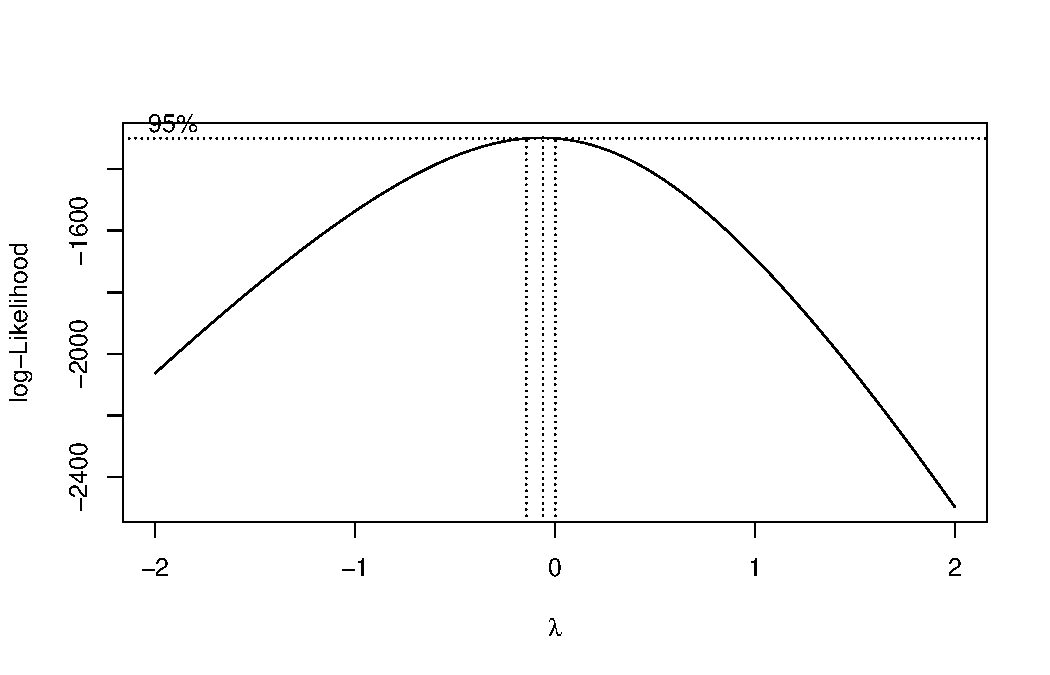
\includegraphics{figure/unnamed-chunk-38-1.pdf}

\begin{itemize}
\tightlist
\item
  Big positive autocorrelation at 1 year (strong seasonal effect)
\item
  Small negative autocorrelation at 1 and 2 months.
\end{itemize}

\end{frame}

\begin{frame}[fragile]{Moving average}
\protect\hypertarget{moving-average}{}

\begin{itemize}
\item
  A particular type of time series called a \textbf{moving average} or
  MA process captures idea of autocorrelations at a few lags but not at
  others.
\item
  Here's generation of MA(1) process, with autocorrelation at lag 1 but
  not otherwise:
\end{itemize}

\begin{Shaded}
\begin{Highlighting}[]
\NormalTok{beta=}\DecValTok{1}
\KeywordTok{tibble}\NormalTok{(}\DataTypeTok{e=}\KeywordTok{rnorm}\NormalTok{(}\DecValTok{100}\NormalTok{)) }\OperatorTok\StringTok{ }
\StringTok{  }\KeywordTok{mutate}\NormalTok{(}\DataTypeTok{e_lag=}\KeywordTok{lag}\NormalTok{(e)) }\OperatorTok\StringTok{ }
\StringTok{  }\KeywordTok{mutate}\NormalTok{(}\DataTypeTok{y=}\NormalTok{e}\OperatorTok{+}\NormalTok{beta}\OperatorTok{*}\NormalTok{e_lag) }\OperatorTok\StringTok{ }
\StringTok{  }\KeywordTok{mutate}\NormalTok{(}\DataTypeTok{y=}\KeywordTok{ifelse}\NormalTok{(}\KeywordTok{is.na}\NormalTok{(y), }\DecValTok{0}\NormalTok{, y)) ->}\StringTok{ }\NormalTok{ma}
\NormalTok{ma}
\end{Highlighting}
\end{Shaded}

\begin{verbatim}
## # A tibble: 100 x 3
##         e   e_lag      y
##     <dbl>   <dbl>  <dbl>
##  1  0.991  NA      0    
##  2  0.469   0.991  1.46 
##  3  0.535   0.469  1.00 
##  4 -0.244   0.535  0.291
##  5  1.17   -0.244  0.928
##  6 -0.473   1.17   0.699
##  7  1.56   -0.473  1.08 
##  8 -0.355   1.56   1.20 
##  9 -0.400  -0.355 -0.755
## 10 -2.10   -0.400 -2.50 
## # … with 90 more rows
\end{verbatim}

\end{frame}

\begin{frame}[fragile]{Comments}
\protect\hypertarget{comments-4}{}

\begin{itemize}
\tightlist
\item
  \texttt{e} contains independent ``random shocks''.
\item
  Start process at 0.
\item
  Then, each value of the time series has that time's random shock, plus
  a multiple of the last time's random shock.
\item
  \texttt{y{[}i{]}} has shock in common with \texttt{y{[}i-1{]}}; should
  be a lag 1 autocorrelation.
\item
  But \texttt{y{[}i{]}} has no shock in common with \texttt{y{[}i-2{]}},
  so no lag 2 autocorrelation (or beyond).
\end{itemize}

\end{frame}

\begin{frame}[fragile]{ACF for MA(1) process xxx}
\protect\hypertarget{acf-for-ma1-process-xxx}{}

\begin{Shaded}
\begin{Highlighting}[]
\KeywordTok{acf}\NormalTok{(ma}\OperatorTok{$}\NormalTok{y, }\DataTypeTok{plot=}\NormalTok{F, }\DataTypeTok{na.rm=}\NormalTok{T) }\OperatorTok\StringTok{ }\KeywordTok{autoplot}\NormalTok{()}
\end{Highlighting}
\end{Shaded}

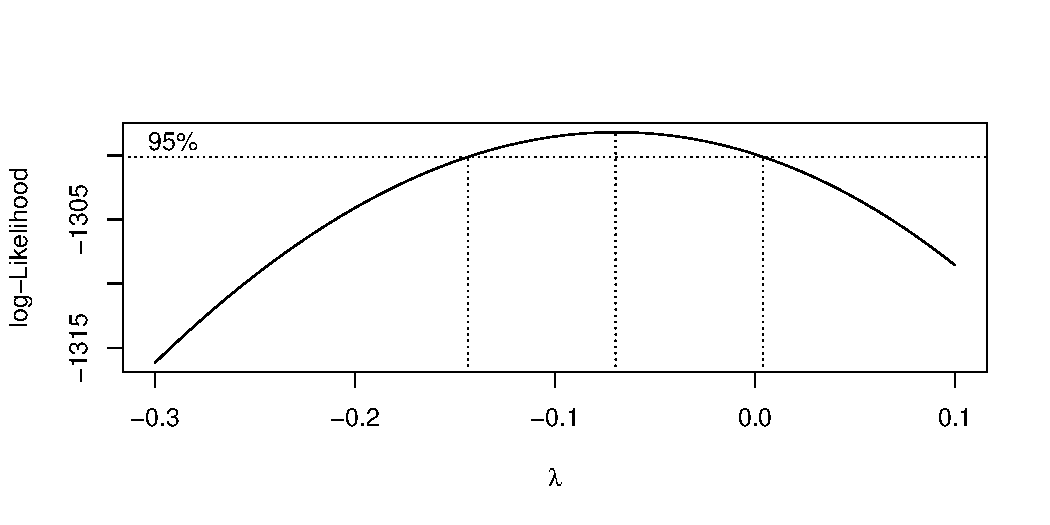
\includegraphics{figure/unnamed-chunk-40-1.pdf}

Everything beyond lag 1 appears to be just chance.

\end{frame}

\begin{frame}[fragile]{AR process}
\protect\hypertarget{ar-process}{}

Another kind of time series is AR process, where each value depends on
previous one, like this (loop):

\begin{Shaded}
\begin{Highlighting}[]
\NormalTok{e=}\KeywordTok{rnorm}\NormalTok{(}\DecValTok{100}\NormalTok{)}
\NormalTok{x=}\KeywordTok{numeric}\NormalTok{(}\DecValTok{0}\NormalTok{)}
\NormalTok{x[}\DecValTok{1}\NormalTok{]=}\DecValTok{0}
\NormalTok{alpha=}\FloatTok{0.7}
\ControlFlowTok{for}\NormalTok{ (i }\ControlFlowTok{in} \DecValTok{2}\OperatorTok{:}\DecValTok{100}\NormalTok{)}
\NormalTok{\{}
\NormalTok{  x[i]=alpha}\OperatorTok{*}\NormalTok{x[i}\DecValTok{-1}\NormalTok{]}\OperatorTok{+}\NormalTok{e[i]}
\NormalTok{\}}
\NormalTok{x}
\end{Highlighting}
\end{Shaded}

\begin{verbatim}
##   [1]  0.00000000  0.69150384 -0.27156693
##   [4] -1.69374385 -0.04624706 -0.61289729
##   [7]  0.26464756 -0.21493841 -1.31429232
##  [10]  0.44277420  0.09918044  0.19080999
##  [13] -1.02379326  0.16693770  0.98374525
##  [16]  0.04866219  1.22331904 -0.04784703
##  [19] -0.21367820 -0.68228901  0.25079396
##  [22] -0.86025292  1.75818244  1.19266409
##  [25]  0.30513461  2.41224530  1.28151011
##  [28]  1.68979182  2.01815565  3.53754507
##  [31]  1.85840920  2.32513921  1.77111656
##  [34]  2.12223993  0.91095776  1.58477201
##  [37]  2.08225425  1.09623045 -0.76369221
##  [40] -0.70809836 -1.84439667 -0.38985352
##  [43] -1.04265756 -0.86988314 -1.14485961
##  [46] -3.18900426 -2.93376468 -2.16075858
##  [49] -1.59508681 -1.74905113 -3.13933449
##  [52] -3.02637272 -1.44218503 -1.55489860
##  [55] -1.73928909 -2.00995900 -2.66272165
##  [58] -3.20337770 -3.51822345 -3.07147301
##  [61] -3.97833623 -3.76371790 -3.52532969
##  [64] -3.45189431 -0.06074526 -0.57178351
##  [67]  0.81558455 -0.27386449  0.75054673
##  [70] -1.41070534 -2.60770962 -0.77008248
##  [73] -0.44599398  0.92659720 -0.50866042
##  [76] -0.28000966 -0.69941661 -0.87488058
##  [79] -1.34524333 -1.24758120 -2.20687436
##  [82] -1.55318855 -0.03079664 -0.30483692
##  [85]  1.32564353  1.13381949  0.88141908
##  [88]  0.19972924 -1.03973656 -0.60655913
##  [91]  0.27269352  0.49555143  0.74140308
##  [94]  0.41684887 -0.01247512 -0.08955967
##  [97]  1.09794055  0.51405840  1.27608083
## [100]  0.05862015
\end{verbatim}

\end{frame}

\begin{frame}[fragile]{Comments}
\protect\hypertarget{comments-5}{}

\begin{itemize}
\tightlist
\item
  Each random shock now only used for its own value of \texttt{x}
\item
  but \texttt{x{[}i{]}} also depends on previous value
  \texttt{x{[}i-1{]}}
\item
  so correlated with previous value
\item
  \emph{but} \texttt{x{[}i{]}} also contains multiple of
  \texttt{x{[}i-2{]}} and previous x's
\item
  so all x's correlated, but autocorrelation dying away.
\end{itemize}

\end{frame}

\begin{frame}[fragile]{ACF for AR(1) series xxx}
\protect\hypertarget{acf-for-ar1-series-xxx}{}

\begin{Shaded}
\begin{Highlighting}[]
\KeywordTok{acf}\NormalTok{(x, }\DataTypeTok{plot=}\NormalTok{F) }\OperatorTok\StringTok{ }\KeywordTok{autoplot}\NormalTok{()}
\end{Highlighting}
\end{Shaded}

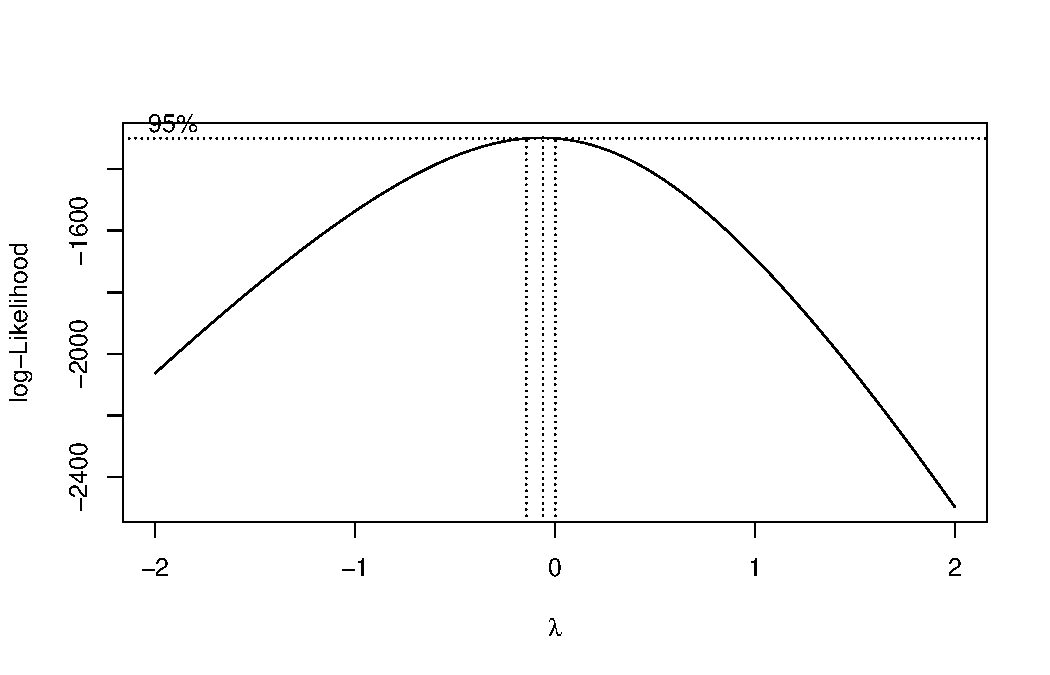
\includegraphics{figure/unnamed-chunk-42-1.pdf}

\end{frame}

\begin{frame}[fragile]{Partial autocorrelation function}
\protect\hypertarget{partial-autocorrelation-function}{}

This cuts off for an AR series: xxx

\begin{Shaded}
\begin{Highlighting}[]
\KeywordTok{pacf}\NormalTok{(x, }\DataTypeTok{plot=}\NormalTok{F) }\OperatorTok\StringTok{ }\KeywordTok{autoplot}\NormalTok{()}
\end{Highlighting}
\end{Shaded}

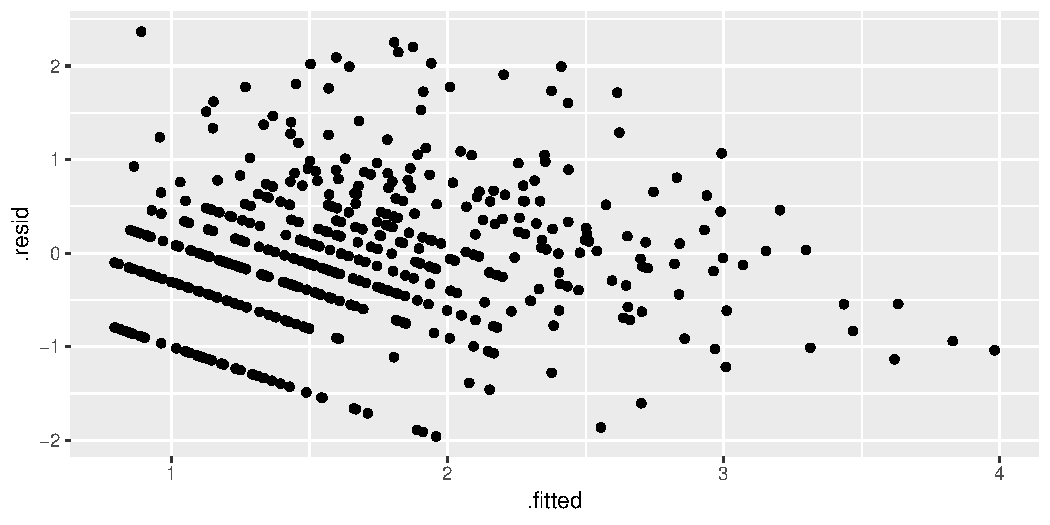
\includegraphics{figure/unnamed-chunk-43-1.pdf}

The lag-2 autocorrelation should not be significant, and isn't.

\end{frame}

\begin{frame}[fragile]{PACF for an MA series decays slowly xxx}
\protect\hypertarget{pacf-for-an-ma-series-decays-slowly-xxx}{}

\begin{Shaded}
\begin{Highlighting}[]
\KeywordTok{pacf}\NormalTok{(ma}\OperatorTok{$}\NormalTok{y, }\DataTypeTok{plot=}\NormalTok{F) }\OperatorTok\StringTok{ }\KeywordTok{autoplot}\NormalTok{()}
\end{Highlighting}
\end{Shaded}

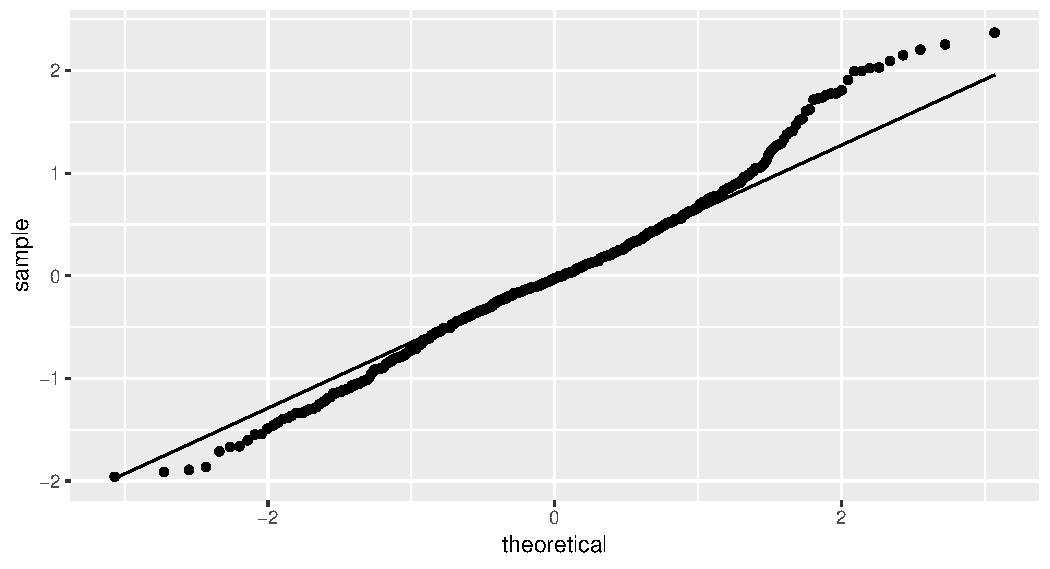
\includegraphics{figure/unnamed-chunk-44-1.pdf}

\end{frame}

\begin{frame}{The old way of doing time series analysis}
\protect\hypertarget{the-old-way-of-doing-time-series-analysis}{}

Starting from a series with constant variability (eg. transform first to
get it, as for souvenirs):

\begin{itemize}
\tightlist
\item
  Assess stationarity.
\item
  If not stationary, take differences as many times as needed until it
  is.
\item
  Look at ACF, see if it dies off. If it does, you have MA series.
\item
  Look at PACF, see if that dies off. If it does, have AR series.
\item
  If neither dies off, probably have a mixed ``ARMA'' series.
\item
  Fit coefficients (like regression slopes).
\item
  Do forecasts.
\end{itemize}

\end{frame}

\begin{frame}[fragile]{The new way of doing time series analysis (in R)}
\protect\hypertarget{the-new-way-of-doing-time-series-analysis-in-r}{}

\begin{itemize}
\tightlist
\item
  Transform series if needed to get constant variability
\item
  Use package \texttt{forecast}.
\item
  Use function \texttt{auto.arima} to estimate what kind of series best
  fits data.
\item
  Use \texttt{forecast} to see what will happen in future.
\end{itemize}

\end{frame}

\begin{frame}[fragile]{Anatomy of \texttt{auto.arima} output}
\protect\hypertarget{anatomy-of-auto.arima-output}{}

\begin{Shaded}
\begin{Highlighting}[]
\KeywordTok{auto.arima}\NormalTok{(ma}\OperatorTok{$}\NormalTok{y)}
\end{Highlighting}
\end{Shaded}

\begin{verbatim}
## Series: ma$y 
## ARIMA(0,0,1) with zero mean 
## 
## Coefficients:
##          ma1
##       0.9070
## s.e.  0.0617
## 
## sigma^2 estimated as 0.9878:  log likelihood=-141.64
## AIC=287.29   AICc=287.41   BIC=292.5
\end{verbatim}

\begin{itemize}
\tightlist
\item
  ARIMA part tells you what kind of series you are estimated to have:

  \begin{itemize}
  \tightlist
  \item
    first number (first 0) is AR (autoregressive) part
  \item
    second number (second 0) is amount of differencing here
  \item
    third number (1) is MA (moving average) part
  \end{itemize}
\item
  Below that, coefficients (with SEs)
\item
  AICc is measure of fit (lower better)
\end{itemize}

\end{frame}

\begin{frame}[fragile]{What other models were possible?}
\protect\hypertarget{what-other-models-were-possible}{}

Run \texttt{auto.arima} with \texttt{trace=T}:

\begin{Shaded}
\begin{Highlighting}[]
\KeywordTok{auto.arima}\NormalTok{(ma}\OperatorTok{$}\NormalTok{y,}\DataTypeTok{trace=}\NormalTok{T)}
\end{Highlighting}
\end{Shaded}

\begin{verbatim}
## 
##  ARIMA(2,0,2) with non-zero mean : Inf
##  ARIMA(0,0,0) with non-zero mean : 345.2328
##  ARIMA(1,0,0) with non-zero mean : 313.9535
##  ARIMA(0,0,1) with non-zero mean : 287.9463
##  ARIMA(0,0,0) with zero mean     : 346.0889
##  ARIMA(1,0,1) with non-zero mean : 290.112
##  ARIMA(0,0,2) with non-zero mean : 290.1128
##  ARIMA(1,0,2) with non-zero mean : 291.7865
##  ARIMA(0,0,1) with zero mean     : 287.4124
##  ARIMA(1,0,1) with zero mean     : 289.4909
##  ARIMA(0,0,2) with zero mean     : 289.4993
##  ARIMA(1,0,0) with zero mean     : 312.7625
##  ARIMA(1,0,2) with zero mean     : 290.6071
## 
##  Best model: ARIMA(0,0,1) with zero mean
\end{verbatim}

\begin{verbatim}
## Series: ma$y 
## ARIMA(0,0,1) with zero mean 
## 
## Coefficients:
##          ma1
##       0.9070
## s.e.  0.0617
## 
## sigma^2 estimated as 0.9878:  log likelihood=-141.64
## AIC=287.29   AICc=287.41   BIC=292.5
\end{verbatim}

Also possible were MA(2) and ARMA(1,1), both with AICc=273.7.

\end{frame}

\begin{frame}[fragile]{Doing it all the new way: white noise}
\protect\hypertarget{doing-it-all-the-new-way-white-noise}{}

\begin{Shaded}
\begin{Highlighting}[]
\NormalTok{wn.aa=}\KeywordTok{auto.arima}\NormalTok{(wn.ts)}
\NormalTok{wn.aa}
\end{Highlighting}
\end{Shaded}

\begin{verbatim}
## Series: wn.ts 
## ARIMA(0,0,0) with zero mean 
## 
## sigma^2 estimated as 1.111:  log likelihood=-147.16
## AIC=296.32   AICc=296.36   BIC=298.93
\end{verbatim}

Best fit \emph{is} white noise (no AR, no MA, no differencing).

\end{frame}

\begin{frame}[fragile]{Forecasts:}
\protect\hypertarget{forecasts}{}

\begin{Shaded}
\begin{Highlighting}[]
\KeywordTok{forecast}\NormalTok{(wn.aa)}
\end{Highlighting}
\end{Shaded}

\begin{verbatim}
##     Point Forecast     Lo 80    Hi 80     Lo 95
## 101              0 -1.350869 1.350869 -2.065975
## 102              0 -1.350869 1.350869 -2.065975
## 103              0 -1.350869 1.350869 -2.065975
## 104              0 -1.350869 1.350869 -2.065975
## 105              0 -1.350869 1.350869 -2.065975
## 106              0 -1.350869 1.350869 -2.065975
## 107              0 -1.350869 1.350869 -2.065975
## 108              0 -1.350869 1.350869 -2.065975
## 109              0 -1.350869 1.350869 -2.065975
## 110              0 -1.350869 1.350869 -2.065975
##        Hi 95
## 101 2.065975
## 102 2.065975
## 103 2.065975
## 104 2.065975
## 105 2.065975
## 106 2.065975
## 107 2.065975
## 108 2.065975
## 109 2.065975
## 110 2.065975
\end{verbatim}

Forecasts all 0, since the past doesn't help to predict future.

\end{frame}

\begin{frame}[fragile]{MA(1)}
\protect\hypertarget{ma1}{}

\begin{Shaded}
\begin{Highlighting}[]
\NormalTok{y.aa=}\KeywordTok{auto.arima}\NormalTok{(ma}\OperatorTok{$}\NormalTok{y)}
\NormalTok{y.aa}
\end{Highlighting}
\end{Shaded}

\begin{verbatim}
## Series: ma$y 
## ARIMA(0,0,1) with zero mean 
## 
## Coefficients:
##          ma1
##       0.9070
## s.e.  0.0617
## 
## sigma^2 estimated as 0.9878:  log likelihood=-141.64
## AIC=287.29   AICc=287.41   BIC=292.5
\end{verbatim}

\begin{Shaded}
\begin{Highlighting}[]
\NormalTok{y.f=}\KeywordTok{forecast}\NormalTok{(y.aa)}
\end{Highlighting}
\end{Shaded}

\end{frame}

\begin{frame}[fragile]{Plotting the forecasts for MA(1) xxx}
\protect\hypertarget{plotting-the-forecasts-for-ma1-xxx}{}

\begin{Shaded}
\begin{Highlighting}[]
\KeywordTok{autoplot}\NormalTok{(y.f)}
\end{Highlighting}
\end{Shaded}

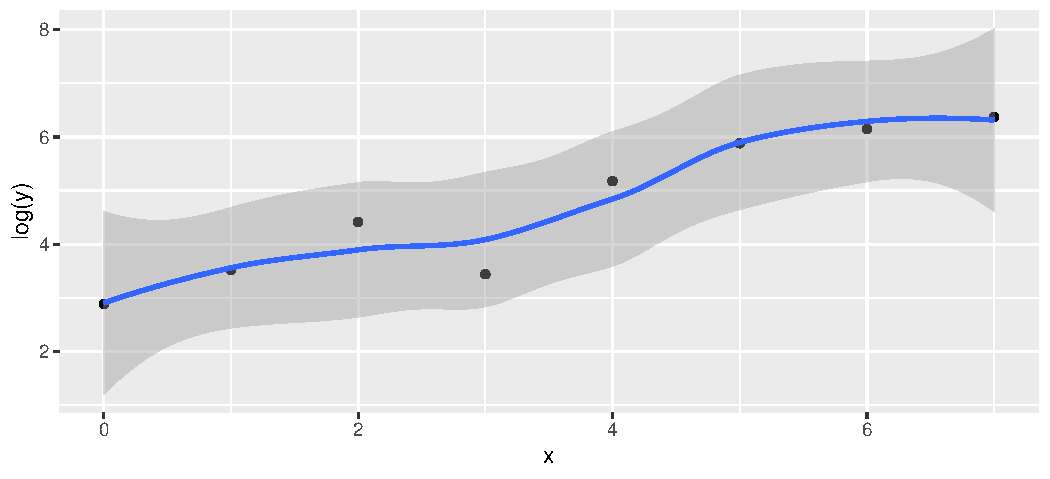
\includegraphics{figure/unnamed-chunk-50-1.pdf}

\end{frame}

\begin{frame}[fragile]{AR(1)}
\protect\hypertarget{ar1}{}

\begin{Shaded}
\begin{Highlighting}[]
\NormalTok{x.aa=}\KeywordTok{auto.arima}\NormalTok{(x)}
\NormalTok{x.aa}
\end{Highlighting}
\end{Shaded}

\begin{verbatim}
## Series: x 
## ARIMA(0,1,1) 
## 
## Coefficients:
##           ma1
##       -0.3544
## s.e.   0.1062
## 
## sigma^2 estimated as 0.979:  log likelihood=-138.99
## AIC=281.97   AICc=282.1   BIC=287.16
\end{verbatim}

Oops!

\end{frame}

\begin{frame}[fragile]{Got it wrong! Fit right AR(1) model:}
\protect\hypertarget{got-it-wrong-fit-right-ar1-model}{}

\begin{Shaded}
\begin{Highlighting}[]
\NormalTok{x.arima=}\KeywordTok{arima}\NormalTok{(x,}\DataTypeTok{order=}\KeywordTok{c}\NormalTok{(}\DecValTok{1}\NormalTok{,}\DecValTok{0}\NormalTok{,}\DecValTok{0}\NormalTok{))}
\NormalTok{x.arima}
\end{Highlighting}
\end{Shaded}

\begin{verbatim}
## 
## Call:
## arima(x = x, order = c(1, 0, 0))
## 
## Coefficients:
##          ar1  intercept
##       0.7758    -0.3646
## s.e.  0.0611     0.4220
## 
## sigma^2 estimated as 0.957:  log likelihood = -140.16,  aic = 286.31
\end{verbatim}

\end{frame}

\begin{frame}[fragile]{Forecasts for \texttt{x} xxx}
\protect\hypertarget{forecasts-for-x-xxx}{}

\begin{Shaded}
\begin{Highlighting}[]
\KeywordTok{forecast}\NormalTok{(x.arima) }\OperatorTok\StringTok{ }\KeywordTok{autoplot}\NormalTok{()}
\end{Highlighting}
\end{Shaded}

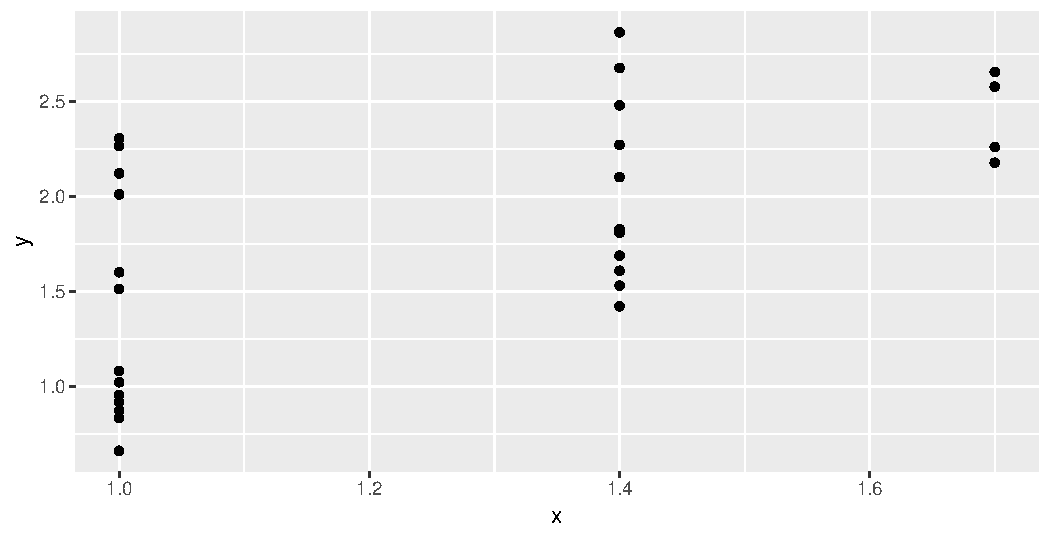
\includegraphics{figure/unnamed-chunk-53-1.pdf}

Comparing wrong model: xxx

\begin{Shaded}
\begin{Highlighting}[]
\KeywordTok{forecast}\NormalTok{(x.aa) }\OperatorTok\StringTok{ }\KeywordTok{autoplot}\NormalTok{()}
\end{Highlighting}
\end{Shaded}

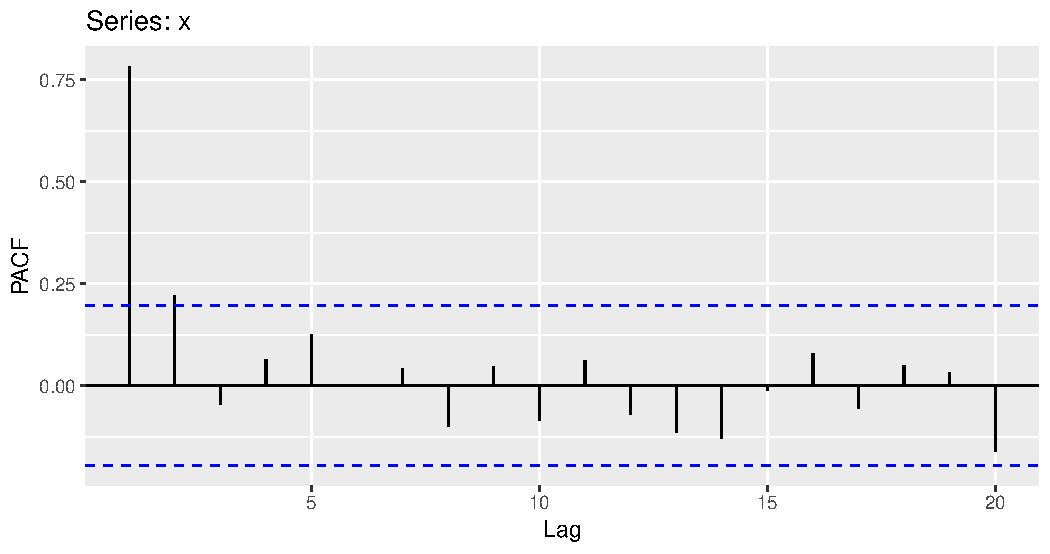
\includegraphics{figure/unnamed-chunk-54-1.pdf}

\end{frame}

\begin{frame}[fragile]{Kings}
\protect\hypertarget{kings}{}

\begin{Shaded}
\begin{Highlighting}[]
\NormalTok{kings.aa=}\KeywordTok{auto.arima}\NormalTok{(kings.ts)}
\NormalTok{kings.aa}
\end{Highlighting}
\end{Shaded}

\begin{verbatim}
## Series: kings.ts 
## ARIMA(0,1,1) 
## 
## Coefficients:
##           ma1
##       -0.7218
## s.e.   0.1208
## 
## sigma^2 estimated as 236.2:  log likelihood=-170.06
## AIC=344.13   AICc=344.44   BIC=347.56
\end{verbatim}

\end{frame}

\begin{frame}[fragile]{Kings forecasts:}
\protect\hypertarget{kings-forecasts}{}

\begin{Shaded}
\begin{Highlighting}[]
\NormalTok{kings.f=}\KeywordTok{forecast}\NormalTok{(kings.aa)}
\NormalTok{kings.f}
\end{Highlighting}
\end{Shaded}

\begin{verbatim}
##    Point Forecast    Lo 80    Hi 80    Lo 95
## 43       67.75063 48.05479 87.44646 37.62845
## 44       67.75063 47.30662 88.19463 36.48422
## 45       67.75063 46.58489 88.91637 35.38042
## 46       67.75063 45.88696 89.61429 34.31304
## 47       67.75063 45.21064 90.29062 33.27869
## 48       67.75063 44.55402 90.94723 32.27448
## 49       67.75063 43.91549 91.58577 31.29793
## 50       67.75063 43.29362 92.20763 30.34687
## 51       67.75063 42.68718 92.81408 29.41939
## 52       67.75063 42.09507 93.40619 28.51383
##        Hi 95
## 43  97.87281
## 44  99.01703
## 45 100.12084
## 46 101.18822
## 47 102.22257
## 48 103.22678
## 49 104.20333
## 50 105.15439
## 51 106.08187
## 52 106.98742
\end{verbatim}

\end{frame}

\begin{frame}[fragile]{Kings forecasts, plotted xxx}
\protect\hypertarget{kings-forecasts-plotted-xxx}{}

\begin{Shaded}
\begin{Highlighting}[]
\KeywordTok{autoplot}\NormalTok{(kings.f) }\OperatorTok{+}\StringTok{ }\KeywordTok{labs}\NormalTok{(}\DataTypeTok{x=}\StringTok{"index"}\NormalTok{, }\DataTypeTok{y=} \StringTok{"age at death"}\NormalTok{)}
\end{Highlighting}
\end{Shaded}

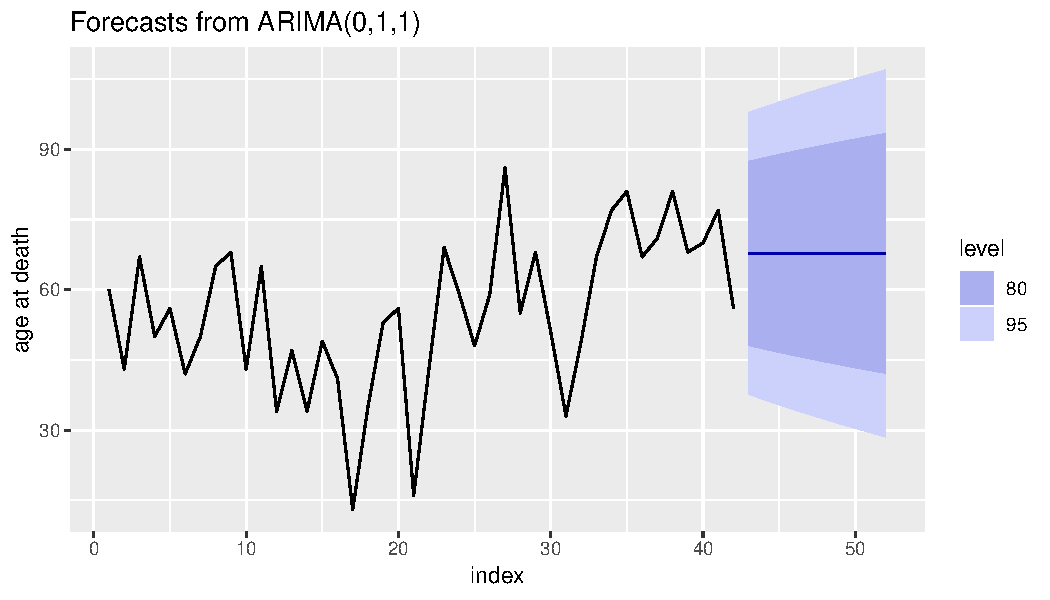
\includegraphics{figure/unnamed-chunk-57-1.pdf}

\end{frame}

\begin{frame}[fragile]{NY births}
\protect\hypertarget{ny-births}{}

\begin{Shaded}
\begin{Highlighting}[]
\NormalTok{ny.aa=}\KeywordTok{auto.arima}\NormalTok{(ny.ts)}
\NormalTok{ny.aa}
\end{Highlighting}
\end{Shaded}

\begin{verbatim}
## Series: ny.ts 
## ARIMA(2,1,2)(1,1,1)[12] 
## 
## Coefficients:
##          ar1      ar2      ma1     ma2     sar1
##       0.6539  -0.4540  -0.7255  0.2532  -0.2427
## s.e.  0.3003   0.2429   0.3227  0.2878   0.0985
##          sma1
##       -0.8451
## s.e.   0.0995
## 
## sigma^2 estimated as 0.4076:  log likelihood=-157.45
## AIC=328.91   AICc=329.67   BIC=350.21
\end{verbatim}

\begin{Shaded}
\begin{Highlighting}[]
\NormalTok{ny.f=}\KeywordTok{forecast}\NormalTok{(ny.aa,}\DataTypeTok{h=}\DecValTok{36}\NormalTok{)}
\end{Highlighting}
\end{Shaded}

Going 36 time periods (3 years) into future.

\end{frame}

\begin{frame}[fragile]{NY births forecasts}
\protect\hypertarget{ny-births-forecasts}{}

Not \emph{quite} same every year:

\begin{Shaded}
\begin{Highlighting}[]
\NormalTok{ny.f}
\end{Highlighting}
\end{Shaded}

\begin{verbatim}
##          Point Forecast    Lo 80    Hi 80    Lo 95
## Jan 1960       27.69056 26.87069 28.51043 26.43668
## Feb 1960       26.07680 24.95838 27.19522 24.36632
## Mar 1960       29.26544 28.01566 30.51523 27.35406
## Apr 1960       27.59444 26.26555 28.92333 25.56208
## May 1960       28.93193 27.52089 30.34298 26.77392
## Jun 1960       28.55379 27.04381 30.06376 26.24448
## Jul 1960       29.84713 28.23370 31.46056 27.37960
## Aug 1960       29.45347 27.74562 31.16132 26.84155
## Sep 1960       29.16388 27.37259 30.95517 26.42433
## Oct 1960       29.21343 27.34498 31.08188 26.35588
## Nov 1960       27.26221 25.31879 29.20563 24.29000
## Dec 1960       28.06863 26.05137 30.08589 24.98349
## Jan 1961       27.66908 25.59684 29.74132 24.49986
## Feb 1961       26.21255 24.08615 28.33895 22.96051
## Mar 1961       29.22612 27.04347 31.40878 25.88804
## Apr 1961       27.58011 25.34076 29.81945 24.15533
## May 1961       28.71354 26.41925 31.00783 25.20473
## Jun 1961       28.21736 25.87042 30.56429 24.62803
## Jul 1961       29.98728 27.58935 32.38521 26.31996
## Aug 1961       29.96127 27.51330 32.40925 26.21743
## Sep 1961       29.56515 27.06786 32.06243 25.74588
## Oct 1961       29.54543 26.99965 32.09121 25.65200
## Nov 1961       27.57845 24.98510 30.17181 23.61226
## Dec 1961       28.40796 25.76792 31.04801 24.37036
## Jan 1962       28.05431 25.33756 30.77106 23.89939
## Feb 1962       26.55936 23.77074 29.34799 22.29453
## Mar 1962       29.61570 26.76474 32.46667 25.25553
## Apr 1962       27.96392 25.05574 30.87209 23.51624
## May 1962       29.14695 26.18187 32.11202 24.61226
## Jun 1962       28.67933 25.65625 31.70240 24.05593
## Jul 1962       30.33348 27.25244 33.41453 25.62143
## Aug 1962       30.21822 27.08057 33.35587 25.41960
## Sep 1962       29.84798 26.65540 33.04056 24.96535
## Oct 1962       29.84511 26.59882 33.09139 24.88034
## Nov 1962       27.88196 24.58270 31.18121 22.83618
## Dec 1962       28.70585 25.35420 32.05750 23.57995
##             Hi 95
## Jan 1960 28.94444
## Feb 1960 27.78728
## Mar 1960 31.17683
## Apr 1960 29.62680
## May 1960 31.08995
## Jun 1960 30.86309
## Jul 1960 32.31466
## Aug 1960 32.06539
## Sep 1960 31.90342
## Oct 1960 32.07098
## Nov 1960 30.23441
## Dec 1960 31.15377
## Jan 1961 30.83830
## Feb 1961 29.46460
## Mar 1961 32.56420
## Apr 1961 31.00488
## May 1961 32.22235
## Jun 1961 31.80668
## Jul 1961 33.65460
## Aug 1961 33.70512
## Sep 1961 33.38441
## Oct 1961 33.43886
## Nov 1961 31.54465
## Dec 1961 32.44556
## Jan 1962 32.20922
## Feb 1962 30.82420
## Mar 1962 33.97588
## Apr 1962 32.41159
## May 1962 33.68164
## Jun 1962 33.30272
## Jul 1962 35.04554
## Aug 1962 35.01684
## Sep 1962 34.73061
## Oct 1962 34.80987
## Nov 1962 32.92773
## Dec 1962 33.83176
\end{verbatim}

\end{frame}

\begin{frame}[fragile]{Plotting the forecasts xxx}
\protect\hypertarget{plotting-the-forecasts-xxx}{}

\begin{Shaded}
\begin{Highlighting}[]
\KeywordTok{autoplot}\NormalTok{(ny.f)}\OperatorTok{+}\KeywordTok{labs}\NormalTok{(}\DataTypeTok{x=}\StringTok{"time"}\NormalTok{, }\DataTypeTok{y=}\StringTok{"births"}\NormalTok{)}
\end{Highlighting}
\end{Shaded}

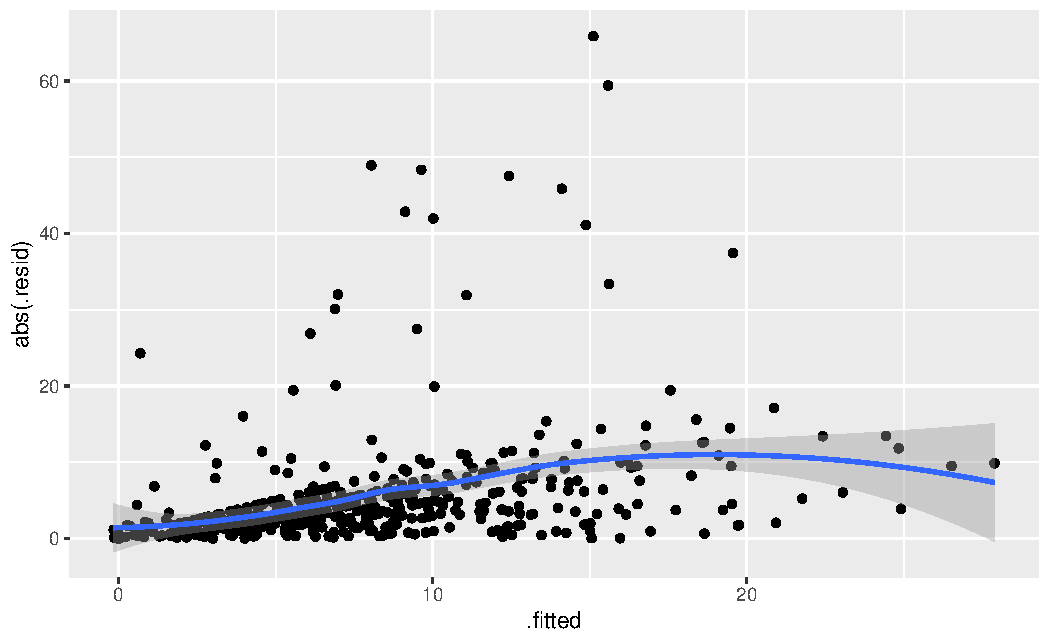
\includegraphics{figure/unnamed-chunk-60-1.pdf}

\end{frame}

\begin{frame}[fragile]{Log-souvenir sales}
\protect\hypertarget{log-souvenir-sales}{}

\begin{Shaded}
\begin{Highlighting}[]
\NormalTok{souv.aa=}\KeywordTok{auto.arima}\NormalTok{(souv.log.ts)}
\NormalTok{souv.aa}
\end{Highlighting}
\end{Shaded}

\begin{verbatim}
## Series: souv.log.ts 
## ARIMA(2,0,0)(0,1,1)[12] with drift 
## 
## Coefficients:
##          ar1     ar2     sma1   drift
##       0.3470  0.3516  -0.5205  0.0238
## s.e.  0.1092  0.1115   0.1700  0.0031
## 
## sigma^2 estimated as 0.02953:  log likelihood=24.54
## AIC=-39.09   AICc=-38.18   BIC=-27.71
\end{verbatim}

\begin{Shaded}
\begin{Highlighting}[]
\NormalTok{souv.f=}\KeywordTok{forecast}\NormalTok{(souv.aa,}\DataTypeTok{h=}\DecValTok{27}\NormalTok{)}
\end{Highlighting}
\end{Shaded}

\end{frame}

\begin{frame}[fragile]{The forecasts}
\protect\hypertarget{the-forecasts}{}

Differenced series showed low value for January (large drop). December
highest, Jan and Feb lowest:

\begin{Shaded}
\begin{Highlighting}[]
\NormalTok{souv.f}
\end{Highlighting}
\end{Shaded}

\begin{verbatim}
##          Point Forecast     Lo 80     Hi 80
## Jan 1994       9.578291  9.358036  9.798545
## Feb 1994       9.754836  9.521700  9.987972
## Mar 1994      10.286195 10.030937 10.541453
## Apr 1994      10.028630  9.765727 10.291532
## May 1994       9.950862  9.681555 10.220168
## Jun 1994      10.116930  9.844308 10.389551
## Jul 1994      10.369140 10.094251 10.644028
## Aug 1994      10.460050 10.183827 10.736274
## Sep 1994      10.535595 10.258513 10.812677
## Oct 1994      10.585995 10.308386 10.863604
## Nov 1994      11.017734 10.739793 11.295674
## Dec 1994      11.795964 11.517817 12.074111
## Jan 1995       9.840884  9.540241 10.141527
## Feb 1995      10.015540  9.711785 10.319295
## Mar 1995      10.555070 10.246346 10.863794
## Apr 1995      10.299676  9.989043 10.610309
## May 1995      10.225535  9.913326 10.537743
## Jun 1995      10.393625 10.080573 10.706676
## Jul 1995      10.647811 10.334184 10.961437
## Aug 1995      10.740118 10.426149 11.054086
## Sep 1995      10.816842 10.502654 11.131031
## Oct 1995      10.868142 10.553818 11.182466
## Nov 1995      11.300608 10.986200 11.615017
## Dec 1995      12.079407 11.764946 12.393869
## Jan 1996      10.124780  9.791571 10.457989
## Feb 1996      10.299793  9.964159 10.635427
## Mar 1996      10.839607 10.499858 11.179355
##              Lo 95     Hi 95
## Jan 1994  9.241440  9.915141
## Feb 1994  9.398285 10.111386
## Mar 1994  9.895811 10.676578
## Apr 1994  9.626555 10.430704
## May 1994  9.538993 10.362731
## Jun 1994  9.699991 10.533868
## Jul 1994  9.948734 10.789545
## Aug 1994 10.037603 10.882498
## Sep 1994 10.111835 10.959356
## Oct 1994 10.161429 11.010561
## Nov 1994 10.592660 11.442807
## Dec 1994 11.370575 12.221353
## Jan 1995  9.381090 10.300678
## Feb 1995  9.550987 10.480093
## Mar 1995 10.082918 11.027222
## Apr 1995  9.824604 10.774749
## May 1995  9.748053 10.703017
## Jun 1995  9.914853 10.872396
## Jul 1995 10.168160 11.127461
## Aug 1995 10.259944 11.220291
## Sep 1995 10.336333 11.297352
## Oct 1995 10.387425 11.348859
## Nov 1995 10.819762 11.781454
## Dec 1995 11.598481 12.560334
## Jan 1996  9.615181 10.634379
## Feb 1996  9.786485 10.813101
## Mar 1996 10.320006 11.359207
\end{verbatim}

\begin{Shaded}
\begin{Highlighting}[]
\NormalTok{souv.f}\OperatorTok{$}\NormalTok{mean}
\end{Highlighting}
\end{Shaded}

\begin{verbatim}
##            Jan       Feb       Mar       Apr
## 1994  9.578291  9.754836 10.286195 10.028630
## 1995  9.840884 10.015540 10.555070 10.299676
## 1996 10.124780 10.299793 10.839607          
##            May       Jun       Jul       Aug
## 1994  9.950862 10.116930 10.369140 10.460050
## 1995 10.225535 10.393625 10.647811 10.740118
## 1996                                        
##            Sep       Oct       Nov       Dec
## 1994 10.535595 10.585995 11.017734 11.795964
## 1995 10.816842 10.868142 11.300608 12.079407
## 1996
\end{verbatim}

\begin{Shaded}
\begin{Highlighting}[]
\KeywordTok{exp}\NormalTok{(souv.f}\OperatorTok{$}\NormalTok{mean)}
\end{Highlighting}
\end{Shaded}

\begin{verbatim}
##            Jan       Feb       Mar       Apr
## 1994  14447.70  17237.39  29324.97  22666.19
## 1995  18786.31  22371.43  38371.49  29723.00
## 1996  24953.76  29726.47  51001.31          
##            May       Jun       Jul       Aug
## 1994  20970.29  24758.64  31861.05  34893.30
## 1995  27599.00  32650.80  42100.33  46171.49
## 1996                                        
##            Sep       Oct       Nov       Dec
## 1994  37631.45  39576.66  60945.41 132715.66
## 1995  49853.43  52477.62  80870.81 176205.71
## 1996
\end{verbatim}

\begin{Shaded}
\begin{Highlighting}[]
\KeywordTok{print.default}\NormalTok{(souv.f)}
\end{Highlighting}
\end{Shaded}

\begin{verbatim}
## $method
## [1] "ARIMA(2,0,0)(0,1,1)[12] with drift"
## 
## $model
## Series: souv.log.ts 
## ARIMA(2,0,0)(0,1,1)[12] with drift 
## 
## Coefficients:
##          ar1     ar2     sma1   drift
##       0.3470  0.3516  -0.5205  0.0238
## s.e.  0.1092  0.1115   0.1700  0.0031
## 
## sigma^2 estimated as 0.02953:  log likelihood=24.54
## AIC=-39.09   AICc=-38.18   BIC=-27.71
## 
## $level
## [1] 80 95
## 
## $mean
##            Jan       Feb       Mar       Apr
## 1994  9.578291  9.754836 10.286195 10.028630
## 1995  9.840884 10.015540 10.555070 10.299676
## 1996 10.124780 10.299793 10.839607          
##            May       Jun       Jul       Aug
## 1994  9.950862 10.116930 10.369140 10.460050
## 1995 10.225535 10.393625 10.647811 10.740118
## 1996                                        
##            Sep       Oct       Nov       Dec
## 1994 10.535595 10.585995 11.017734 11.795964
## 1995 10.816842 10.868142 11.300608 12.079407
## 1996                                        
## 
## $lower
##                80%       95%
## Jan 1994  9.358036  9.241440
## Feb 1994  9.521700  9.398285
## Mar 1994 10.030937  9.895811
## Apr 1994  9.765727  9.626555
## May 1994  9.681555  9.538993
## Jun 1994  9.844308  9.699991
## Jul 1994 10.094251  9.948734
## Aug 1994 10.183827 10.037603
## Sep 1994 10.258513 10.111835
## Oct 1994 10.308386 10.161429
## Nov 1994 10.739793 10.592660
## Dec 1994 11.517817 11.370575
## Jan 1995  9.540241  9.381090
## Feb 1995  9.711785  9.550987
## Mar 1995 10.246346 10.082918
## Apr 1995  9.989043  9.824604
## May 1995  9.913326  9.748053
## Jun 1995 10.080573  9.914853
## Jul 1995 10.334184 10.168160
## Aug 1995 10.426149 10.259944
## Sep 1995 10.502654 10.336333
## Oct 1995 10.553818 10.387425
## Nov 1995 10.986200 10.819762
## Dec 1995 11.764946 11.598481
## Jan 1996  9.791571  9.615181
## Feb 1996  9.964159  9.786485
## Mar 1996 10.499858 10.320006
## 
## $upper
##                80%       95%
## Jan 1994  9.798545  9.915141
## Feb 1994  9.987972 10.111386
## Mar 1994 10.541453 10.676578
## Apr 1994 10.291532 10.430704
## May 1994 10.220168 10.362731
## Jun 1994 10.389551 10.533868
## Jul 1994 10.644028 10.789545
## Aug 1994 10.736274 10.882498
## Sep 1994 10.812677 10.959356
## Oct 1994 10.863604 11.010561
## Nov 1994 11.295674 11.442807
## Dec 1994 12.074111 12.221353
## Jan 1995 10.141527 10.300678
## Feb 1995 10.319295 10.480093
## Mar 1995 10.863794 11.027222
## Apr 1995 10.610309 10.774749
## May 1995 10.537743 10.703017
## Jun 1995 10.706676 10.872396
## Jul 1995 10.961437 11.127461
## Aug 1995 11.054086 11.220291
## Sep 1995 11.131031 11.297352
## Oct 1995 11.182466 11.348859
## Nov 1995 11.615017 11.781454
## Dec 1995 12.393869 12.560334
## Jan 1996 10.457989 10.634379
## Feb 1996 10.635427 10.813101
## Mar 1996 11.179355 11.359207
## 
## $x
##            Jan       Feb       Mar       Apr
## 1987  7.417466  7.782194  7.951809  8.173939
## 1988  7.823970  8.556075  8.885322  8.477627
## 1989  8.458933  8.648683  9.206089  8.576364
## 1990  8.686278  8.668124  9.427164  8.759319
## 1991  8.481906  8.774967  9.173549  9.084910
## 1992  8.937879  9.195195  9.585923  9.357668
## 1993  9.234373  9.329623  9.990896  9.761770
##            May       Jun       Jul       Aug
## 1987  8.230300  8.220064  8.377841  8.179295
## 1988  8.682857  8.507414  8.728931  8.466352
## 1989  8.778392  8.799481  8.902404  9.009034
## 1990  8.937103  8.885268  9.002236  8.984600
## 1991  9.073646  9.231072  9.330481  9.437653
## 1992  9.141265  9.478999  9.725125  9.897902
## 1993  9.680206  9.830999 10.171801 10.260691
##            Sep       Oct       Nov       Dec
## 1987  8.521548  8.767715  8.935982  9.891223
## 1988  8.611854  8.671647  9.441458 10.259122
## 1989  9.056393  9.178901  9.625877 10.435909
## 1990  8.998762  9.045077  9.793375 10.312759
## 1991  9.361978  9.518332  9.990679 10.715766
## 1992 10.083029 10.142164 10.491963 11.298763
## 1993 10.325659 10.335962 10.750093 11.558479
## 
## $series
## [1] "souv.log.ts"
## 
## $fitted
##            Jan       Feb       Mar       Apr
## 1987  7.410073  7.774460  7.943929  8.165861
## 1988  7.737469  8.200398  8.494420  8.807962
## 1989  8.209173  8.832180  9.049762  8.851068
## 1990  8.548108  8.966186  9.300665  8.884112
## 1991  8.716867  8.794359  9.412746  8.860024
## 1992  8.899194  9.171104  9.689975  9.345013
## 1993  9.382292  9.576494  9.877050  9.624983
##            May       Jun       Jul       Aug
## 1987  8.222189  8.211987  8.369630  8.171306
## 1988  8.735935  8.554636  8.713493  8.472167
## 1989  8.934449  8.684461  8.939090  8.722942
## 1990  9.083565  8.946289  9.091940  9.015035
## 1991  9.122753  9.165059  9.302968  9.322395
## 1992  9.424726  9.402271  9.512202  9.688090
## 1993  9.657431  9.854253 10.012085 10.153607
##            Sep       Oct       Nov       Dec
## 1987  8.513240  8.759186  8.927308  9.881618
## 1988  8.791805  8.929755  9.050992 10.081222
## 1989  9.025778  9.214826  9.667959 10.502318
## 1990  9.152643  9.253725  9.667494 10.566558
## 1991  9.437171  9.524619 10.106639 10.765163
## 1992  9.785742 10.019754 10.606887 11.220778
## 1993 10.297393 10.376320 10.790406 11.502027
## 
## $residuals
##               Jan          Feb          Mar
## 1987  0.007393658  0.007734578  0.007880384
## 1988  0.086500680  0.355677770  0.390902029
## 1989  0.249759758 -0.183497442  0.156327204
## 1990  0.138169613 -0.298061978  0.126498707
## 1991 -0.234960761 -0.019392105 -0.239197642
## 1992  0.038684952  0.024091125 -0.104051475
## 1993 -0.147918881 -0.246870842  0.113845932
##               Apr          May          Jun
## 1987  0.008078708  0.008111263  0.008077223
## 1988 -0.330335699 -0.053078628 -0.047222006
## 1989 -0.274704599 -0.156057171  0.115019554
## 1990 -0.124793133 -0.146462326 -0.061020897
## 1991  0.224886129 -0.049106990  0.066013439
## 1992  0.012654844 -0.283461096  0.076727977
## 1993  0.136787334  0.022775020 -0.023253788
##               Jul          Aug          Sep
## 1987  0.008211198  0.007988850  0.008307302
## 1988  0.015437982 -0.005814548 -0.179950487
## 1989 -0.036685983  0.286092365  0.030614769
## 1990 -0.089703878 -0.030435015 -0.153880639
## 1991  0.027512770  0.115258184 -0.075192996
## 1992  0.212922849  0.209812963  0.297287851
## 1993  0.159715936  0.107083958  0.028266617
##               Oct          Nov          Dec
## 1987  0.008529669  0.008674137  0.009605578
## 1988 -0.258107829  0.390466497  0.177900145
## 1989 -0.035925124 -0.042081989 -0.066409363
## 1990 -0.208648543  0.125880605 -0.253799233
## 1991 -0.006287476 -0.115960322 -0.049397837
## 1992  0.122410050 -0.114924058  0.077984541
## 1993 -0.040357792 -0.040312585  0.056451584
## 
## attr(,"class")
## [1] "forecast"
\end{verbatim}

\end{frame}

\begin{frame}[fragile]{Plotting the forecasts xxx}
\protect\hypertarget{plotting-the-forecasts-xxx-1}{}

\begin{Shaded}
\begin{Highlighting}[]
\KeywordTok{autoplot}\NormalTok{(souv.f)}
\end{Highlighting}
\end{Shaded}

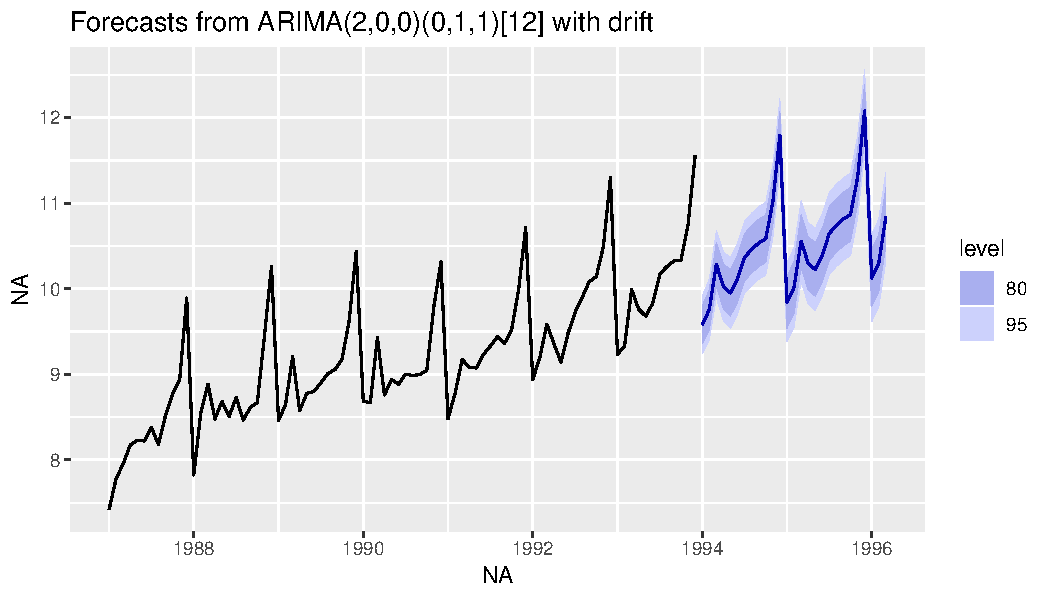
\includegraphics{figure/unnamed-chunk-63-1.pdf}

\end{frame}

\begin{frame}[fragile]{Global mean temperatures, revisited}
\protect\hypertarget{global-mean-temperatures-revisited}{}

\begin{Shaded}
\begin{Highlighting}[]
\NormalTok{temp.ts=}\KeywordTok{ts}\NormalTok{(temp}\OperatorTok{$}\NormalTok{temperature,}\DataTypeTok{start=}\DecValTok{1880}\NormalTok{)}
\NormalTok{temp.aa=}\KeywordTok{auto.arima}\NormalTok{(temp.ts)}
\NormalTok{temp.aa}
\end{Highlighting}
\end{Shaded}

\begin{verbatim}
## Series: temp.ts 
## ARIMA(1,1,3) with drift 
## 
## Coefficients:
##           ar1     ma1      ma2      ma3   drift
##       -0.9374  0.5038  -0.6320  -0.2988  0.0067
## s.e.   0.0835  0.1088   0.0876   0.0844  0.0025
## 
## sigma^2 estimated as 0.008939:  log likelihood=124.34
## AIC=-236.67   AICc=-235.99   BIC=-219.47
\end{verbatim}

\end{frame}

\begin{frame}[fragile]{Forecasts xxx}
\protect\hypertarget{forecasts-xxx}{}

\begin{Shaded}
\begin{Highlighting}[]
\NormalTok{temp.f=}\KeywordTok{forecast}\NormalTok{(temp.aa)}
\KeywordTok{autoplot}\NormalTok{(temp.f)}\OperatorTok{+}\KeywordTok{labs}\NormalTok{(}\DataTypeTok{x=}\StringTok{"year"}\NormalTok{, }\DataTypeTok{y=}\StringTok{"temperature"}\NormalTok{)}
\end{Highlighting}
\end{Shaded}

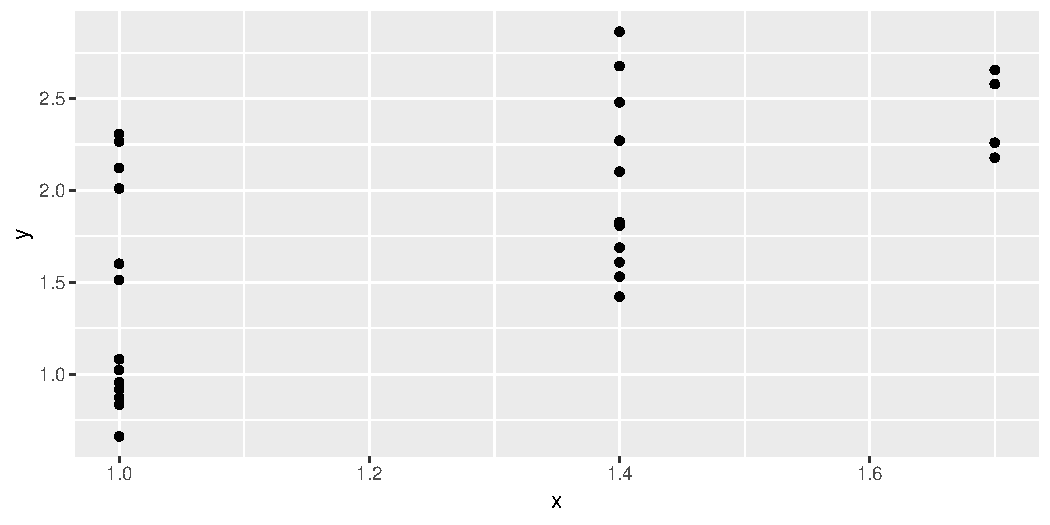
\includegraphics{figure/unnamed-chunk-65-1.pdf}

\end{frame}

\hypertarget{multiway-frequency-tables}{%
\section{Multiway frequency tables}\label{multiway-frequency-tables}}

\begin{frame}[fragile]{Packages}
\protect\hypertarget{packages-1}{}

\begin{Shaded}
\begin{Highlighting}[]
\KeywordTok{library}\NormalTok{(tidyverse)}
\end{Highlighting}
\end{Shaded}

\end{frame}

\begin{frame}{Multi-way frequency analysis}
\protect\hypertarget{multi-way-frequency-analysis}{}

\begin{itemize}
\item
  A study of gender and eyewear-wearing finds the following frequencies:

  \begin{tabular}{lrrr}
  \hline
  Gender & Contacts & Glasses & None \\
  \hline
  Female & 121 & 32 & 129 \\
  Male & 42 & 37 & 85\\
  \hline
  \end{tabular}
\item
  Is there association between eyewear and gender?
\item
  Normally answer this with chisquare test (based on observed and
  expected frequencies from null hypothesis of no association).
\item
  Two categorical variables and a frequency.
\item
  We assess in way that generalizes to more categorical variables.
\end{itemize}

\end{frame}

\begin{frame}[fragile]{The data file}
\protect\hypertarget{the-data-file}{}

\begin{verbatim}

gender contacts glasses none
female 121      32      129
male   42       37      85
\end{verbatim}

\begin{itemize}
\item
  This is \emph{not tidy!}
\item
  Two variables are gender and \emph{eyewear}, and those numbers all
  frequencies.
\end{itemize}

\begin{Shaded}
\begin{Highlighting}[]
\NormalTok{my_url <-}\StringTok{ "http://www.utsc.utoronto.ca/~butler/d29/eyewear.txt"}
\NormalTok{eyewear <-}\StringTok{ }\KeywordTok{read_delim}\NormalTok{(my_url, }\StringTok{" "}\NormalTok{)}
\NormalTok{eyewear}
\end{Highlighting}
\end{Shaded}

\begin{verbatim}
## # A tibble: 2 x 4
##   gender contacts glasses  none
##   <chr>     <dbl>   <dbl> <dbl>
## 1 female      121      32   129
## 2 male         42      37    85
\end{verbatim}

\end{frame}

\begin{frame}[fragile]{Tidying the data}
\protect\hypertarget{tidying-the-data}{}

\begin{Shaded}
\begin{Highlighting}[]
\NormalTok{eyes <-}\StringTok{ }\NormalTok{eyewear }\OperatorTok
\StringTok{  }\KeywordTok{gather}\NormalTok{(eyewear, frequency, contacts}\OperatorTok{:}\NormalTok{none)}
\NormalTok{eyes}
\end{Highlighting}
\end{Shaded}

\begin{verbatim}
## # A tibble: 6 x 3
##   gender eyewear  frequency
##   <chr>  <chr>        <dbl>
## 1 female contacts       121
## 2 male   contacts        42
## 3 female glasses         32
## 4 male   glasses         37
## 5 female none           129
## 6 male   none            85
\end{verbatim}

\begin{Shaded}
\begin{Highlighting}[]
\NormalTok{xt <-}\StringTok{ }\KeywordTok{xtabs}\NormalTok{(frequency }\OperatorTok{~}\StringTok{ }\NormalTok{gender }\OperatorTok{+}\StringTok{ }\NormalTok{eyewear, }\DataTypeTok{data =}\NormalTok{ eyes)}
\NormalTok{xt}
\end{Highlighting}
\end{Shaded}

\begin{verbatim}
##         eyewear
## gender   contacts glasses none
##   female      121      32  129
##   male         42      37   85
\end{verbatim}

\end{frame}

\begin{frame}[fragile]{Modelling}
\protect\hypertarget{modelling}{}

\begin{itemize}
\item
  Last table on previous page is ``reconstituted'' contingency table,
  for checking.
\item
  Predict frequency from other factors and combos. \texttt{glm} with
  \texttt{poisson} family.
\end{itemize}

\begin{Shaded}
\begin{Highlighting}[]
\NormalTok{eyes}\FloatTok{.1}\NormalTok{ <-}\StringTok{ }\KeywordTok{glm}\NormalTok{(frequency }\OperatorTok{~}\StringTok{ }\NormalTok{gender }\OperatorTok{*}\StringTok{ }\NormalTok{eyewear,}
  \DataTypeTok{data =}\NormalTok{ eyes,}
  \DataTypeTok{family =} \StringTok{"poisson"}
\NormalTok{)}
\end{Highlighting}
\end{Shaded}

def

\begin{itemize}
\tightlist
\item
  Called \textbf{log-linear model}.
\end{itemize}

\end{frame}

\begin{frame}[fragile]{What can we get rid of?}
\protect\hypertarget{what-can-we-get-rid-of}{}

\{\small    

\begin{Shaded}
\begin{Highlighting}[]
\KeywordTok{drop1}\NormalTok{(eyes}\FloatTok{.1}\NormalTok{, }\DataTypeTok{test =} \StringTok{"Chisq"}\NormalTok{)}
\end{Highlighting}
\end{Shaded}

\begin{verbatim}
## Single term deletions
## 
## Model:
## frequency ~ gender * eyewear
##                Df Deviance    AIC    LRT  Pr(>Chi)
## <none>               0.000 47.958                 
## gender:eyewear  2   17.829 61.787 17.829 0.0001345
##                   
## <none>            
## gender:eyewear ***
## ---
## Signif. codes:  
## 0 '***' 0.001 '**' 0.01 '*' 0.05 '.' 0.1 ' ' 1
\end{verbatim}

def \}

\end{frame}

\begin{frame}[fragile]{Conclusions}
\protect\hypertarget{conclusions-1}{}

\begin{itemize}
\item
  \texttt{drop1} says what we can remove at this step. Significant =
  must stay.
\item
  Cannot remove anything.
\item
  Frequency depends on \texttt{gender-wear} \emph{combination}, cannot
  be simplified further.
\item
  Gender and eyewear are \emph{associated}.
\item
  Stop here.
\end{itemize}

\end{frame}

\begin{frame}[fragile]{\texttt{prop.table}}
\protect\hypertarget{prop.table}{}

Original table:

\{\footnotesize

\begin{Shaded}
\begin{Highlighting}[]
\NormalTok{xt}
\end{Highlighting}
\end{Shaded}

\begin{verbatim}
##         eyewear
## gender   contacts glasses none
##   female      121      32  129
##   male         42      37   85
\end{verbatim}

\} Calculate eg. row proportions like this:

\{\small

\begin{Shaded}
\begin{Highlighting}[]
\KeywordTok{prop.table}\NormalTok{(xt, }\DataTypeTok{margin =} \DecValTok{1}\NormalTok{)}
\end{Highlighting}
\end{Shaded}

\begin{verbatim}
##         eyewear
## gender    contacts   glasses      none
##   female 0.4290780 0.1134752 0.4574468
##   male   0.2560976 0.2256098 0.5182927
\end{verbatim}

\}

\begin{itemize}
\item
  \texttt{margin} says what to make add to 1.
\item
  More females wear contacts and more males wear glasses.
\end{itemize}

\end{frame}

\begin{frame}[fragile]{No association}
\protect\hypertarget{no-association}{}

\begin{itemize}
\tightlist
\item
  Suppose table had been as shown below:
\end{itemize}

\begin{Shaded}
\begin{Highlighting}[]
\NormalTok{my_url <-}\StringTok{ "http://www.utsc.utoronto.ca/~butler/d29/eyewear2.txt"}
\NormalTok{eyewear2 <-}\StringTok{ }\KeywordTok{read_table}\NormalTok{(my_url)}
\NormalTok{eyes2 <-}\StringTok{ }\NormalTok{eyewear2 }\OperatorTok\StringTok{ }\KeywordTok{gather}\NormalTok{(eyewear, frequency, contacts}\OperatorTok{:}\NormalTok{none)}
\NormalTok{xt2 <-}\StringTok{ }\KeywordTok{xtabs}\NormalTok{(frequency }\OperatorTok{~}\StringTok{ }\NormalTok{gender }\OperatorTok{+}\StringTok{ }\NormalTok{eyewear, }\DataTypeTok{data =}\NormalTok{ eyes2)}
\NormalTok{xt2}
\end{Highlighting}
\end{Shaded}

\begin{verbatim}
##         eyewear
## gender   contacts glasses none
##   female      150      30  120
##   male         75      16   62
\end{verbatim}

\begin{Shaded}
\begin{Highlighting}[]
\KeywordTok{prop.table}\NormalTok{(xt2, }\DataTypeTok{margin =} \DecValTok{1}\NormalTok{)}
\end{Highlighting}
\end{Shaded}

\begin{verbatim}
##         eyewear
## gender    contacts   glasses      none
##   female 0.5000000 0.1000000 0.4000000
##   male   0.4901961 0.1045752 0.4052288
\end{verbatim}

\begin{itemize}
\tightlist
\item
  Females and males wear contacts and glasses in same proportions
  (though more females and more contact-wearers). No \emph{association}
  between gender and eyewear.
\end{itemize}

\end{frame}

\begin{frame}[fragile]{Analysis for revised data}
\protect\hypertarget{analysis-for-revised-data}{}

\begin{Shaded}
\begin{Highlighting}[]
\NormalTok{eyes}\FloatTok{.2}\NormalTok{ <-}\StringTok{ }\KeywordTok{glm}\NormalTok{(frequency }\OperatorTok{~}\StringTok{ }\NormalTok{gender }\OperatorTok{*}\StringTok{ }\NormalTok{eyewear,}
  \DataTypeTok{data =}\NormalTok{ eyes2,}
  \DataTypeTok{family =} \StringTok{"poisson"}
\NormalTok{)}
\KeywordTok{drop1}\NormalTok{(eyes}\FloatTok{.2}\NormalTok{, }\DataTypeTok{test =} \StringTok{"Chisq"}\NormalTok{)}
\end{Highlighting}
\end{Shaded}

\begin{verbatim}
## Single term deletions
## 
## Model:
## frequency ~ gender * eyewear
##                Df Deviance    AIC      LRT Pr(>Chi)
## <none>            0.000000 47.467                  
## gender:eyewear  2 0.047323 43.515 0.047323   0.9766
\end{verbatim}

No longer any association. Take out interaction.

\end{frame}

\begin{frame}[fragile]{No interaction}
\protect\hypertarget{no-interaction}{}

\{\small

\begin{Shaded}
\begin{Highlighting}[]
\NormalTok{eyes}\FloatTok{.3}\NormalTok{ <-}\StringTok{ }\KeywordTok{update}\NormalTok{(eyes}\FloatTok{.2}\NormalTok{, . }\OperatorTok{~}\StringTok{ }\NormalTok{. }\OperatorTok{-}\StringTok{ }\NormalTok{gender}\OperatorTok{:}\NormalTok{eyewear)}
\KeywordTok{drop1}\NormalTok{(eyes}\FloatTok{.3}\NormalTok{, }\DataTypeTok{test =} \StringTok{"Chisq"}\NormalTok{)}
\end{Highlighting}
\end{Shaded}

\begin{verbatim}
## Single term deletions
## 
## Model:
## frequency ~ gender + eyewear
##         Df Deviance     AIC     LRT  Pr(>Chi)    
## <none>        0.047  43.515                      
## gender   1   48.624  90.091  48.577 3.176e-12 ***
## eyewear  2  138.130 177.598 138.083 < 2.2e-16 ***
## ---
## Signif. codes:  
## 0 '***' 0.001 '**' 0.01 '*' 0.05 '.' 0.1 ' ' 1
\end{verbatim}

\}

\begin{itemize}
\item
  More females (gender effect)
\item
  more contact-wearers (eyewear effect)
\item
  no association (no interaction).
\end{itemize}

\end{frame}

\begin{frame}{Chest pain, being overweight and being a smoker}
\protect\hypertarget{chest-pain-being-overweight-and-being-a-smoker}{}

\begin{itemize}
\item
  In a hospital emergency department, 176 subjects who attended for
  acute chest pain took part in a study.
\item
  Each subject had a normal or abnormal electrocardiogram reading (ECG),
  were overweight (as judged by BMI) or not, and were a smoker or not.
\item
  How are these three variables related, or not?
\end{itemize}

\end{frame}

\begin{frame}[fragile]{The data}
\protect\hypertarget{the-data}{}

In modelling-friendly format:

\begin{verbatim}

ecg bmi smoke count
abnormal overweight yes 47
abnormal overweight no 10
abnormal normalweight yes 8 
abnormal normalweight no 6
normal overweight yes 25 
normal overweight no 15 
normal normalweight yes 35
normal normalweight no 30
\end{verbatim}

\end{frame}

\begin{frame}[fragile]{First step}
\protect\hypertarget{first-step}{}

\begin{Shaded}
\begin{Highlighting}[]
\NormalTok{my_url <-}\StringTok{ "http://www.utsc.utoronto.ca/~butler/d29/ecg.txt"}
\NormalTok{chest <-}\StringTok{ }\KeywordTok{read_delim}\NormalTok{(my_url, }\StringTok{" "}\NormalTok{)}
\NormalTok{chest}\FloatTok{.1}\NormalTok{ <-}\StringTok{ }\KeywordTok{glm}\NormalTok{(count }\OperatorTok{~}\StringTok{ }\NormalTok{ecg }\OperatorTok{*}\StringTok{ }\NormalTok{bmi }\OperatorTok{*}\StringTok{ }\NormalTok{smoke,}
  \DataTypeTok{data =}\NormalTok{ chest,}
  \DataTypeTok{family =} \StringTok{"poisson"}
\NormalTok{)}
\KeywordTok{drop1}\NormalTok{(chest}\FloatTok{.1}\NormalTok{, }\DataTypeTok{test =} \StringTok{"Chisq"}\NormalTok{)}
\end{Highlighting}
\end{Shaded}

\begin{verbatim}
## Single term deletions
## 
## Model:
## count ~ ecg * bmi * smoke
##               Df Deviance    AIC    LRT Pr(>Chi)
## <none>             0.0000 53.707                
## ecg:bmi:smoke  1   1.3885 53.096 1.3885   0.2387
\end{verbatim}

That 3-way interaction comes out.

\end{frame}

\begin{frame}[fragile]{Removing the 3-way interaction}
\protect\hypertarget{removing-the-3-way-interaction}{}

\begin{Shaded}
\begin{Highlighting}[]
\NormalTok{chest}\FloatTok{.2}\NormalTok{ <-}\StringTok{ }\KeywordTok{update}\NormalTok{(chest}\FloatTok{.1}\NormalTok{, . }\OperatorTok{~}\StringTok{ }\NormalTok{. }\OperatorTok{-}\StringTok{ }\NormalTok{ecg}\OperatorTok{:}\NormalTok{bmi}\OperatorTok{:}\NormalTok{smoke)}
\KeywordTok{drop1}\NormalTok{(chest}\FloatTok{.2}\NormalTok{, }\DataTypeTok{test =} \StringTok{"Chisq"}\NormalTok{)}
\end{Highlighting}
\end{Shaded}

\begin{verbatim}
## Single term deletions
## 
## Model:
## count ~ ecg + bmi + smoke + ecg:bmi + ecg:smoke + bmi:smoke
##           Df Deviance    AIC     LRT  Pr(>Chi)    
## <none>         1.3885 53.096                      
## ecg:bmi    1  29.0195 78.727 27.6310 1.468e-07 ***
## ecg:smoke  1   4.8935 54.601  3.5050   0.06119 .  
## bmi:smoke  1   4.4689 54.176  3.0803   0.07924 .  
## ---
## Signif. codes:  
## 0 '***' 0.001 '**' 0.01 '*' 0.05 '.' 0.1 ' ' 1
\end{verbatim}

At \(\alpha=0.05\), \texttt{bmi:smoke} comes out.

\end{frame}

\begin{frame}[fragile]{Removing \texttt{bmi:smoke}}
\protect\hypertarget{removing-bmismoke}{}

\begin{Shaded}
\begin{Highlighting}[]
\NormalTok{chest}\FloatTok{.3}\NormalTok{ <-}\StringTok{ }\KeywordTok{update}\NormalTok{(chest}\FloatTok{.2}\NormalTok{, . }\OperatorTok{~}\StringTok{ }\NormalTok{. }\OperatorTok{-}\StringTok{ }\NormalTok{bmi}\OperatorTok{:}\NormalTok{smoke)}
\KeywordTok{drop1}\NormalTok{(chest}\FloatTok{.3}\NormalTok{, }\DataTypeTok{test =} \StringTok{"Chisq"}\NormalTok{)}
\end{Highlighting}
\end{Shaded}

\begin{verbatim}
## Single term deletions
## 
## Model:
## count ~ ecg + bmi + smoke + ecg:bmi + ecg:smoke
##           Df Deviance    AIC    LRT  Pr(>Chi)    
## <none>          4.469 54.176                     
## ecg:bmi    1   36.562 84.270 32.094 1.469e-08 ***
## ecg:smoke  1   12.436 60.144  7.968  0.004762 ** 
## ---
## Signif. codes:  
## 0 '***' 0.001 '**' 0.01 '*' 0.05 '.' 0.1 ' ' 1
\end{verbatim}

\texttt{ecg:smoke} has become significant. So we have to stop.

\end{frame}

\begin{frame}[fragile]{Understanding the final model}
\protect\hypertarget{understanding-the-final-model}{}

\begin{itemize}
\item
  Thinking of \texttt{ecg} as ``response'' that might depend on anything
  else.
\item
  What is associated with \texttt{ecg}? Both \texttt{bmi} on its own and
  \texttt{smoke} on its own, but \emph{not} the combination of both.
\item
  \texttt{ecg:bmi} table:
\end{itemize}

\begin{Shaded}
\begin{Highlighting}[]
\KeywordTok{xtabs}\NormalTok{(count }\OperatorTok{~}\StringTok{ }\NormalTok{ecg }\OperatorTok{+}\StringTok{ }\NormalTok{bmi, }\DataTypeTok{data =}\NormalTok{ chest)}
\end{Highlighting}
\end{Shaded}

\begin{verbatim}
##           bmi
## ecg        normalweight overweight
##   abnormal           14         57
##   normal             65         40
\end{verbatim}

\begin{itemize}
\tightlist
\item
  Most normal weight people have a normal ECG, but a majority of
  overweight people have an \emph{abnormal} ECG. That is, knowing about
  BMI says something about likely ECG.
\end{itemize}

\end{frame}

\begin{frame}[fragile]{\texttt{ecg:smoke}}
\protect\hypertarget{ecgsmoke}{}

\begin{itemize}
\tightlist
\item
  \texttt{ecg:smoke} table:
\end{itemize}

\begin{Shaded}
\begin{Highlighting}[]
\KeywordTok{xtabs}\NormalTok{(count }\OperatorTok{~}\StringTok{ }\NormalTok{ecg }\OperatorTok{+}\StringTok{ }\NormalTok{smoke, }\DataTypeTok{data =}\NormalTok{ chest)}
\end{Highlighting}
\end{Shaded}

\begin{verbatim}
##           smoke
## ecg        no yes
##   abnormal 16  55
##   normal   45  60
\end{verbatim}

\begin{itemize}
\item
  Most nonsmokers have a normal ECG, but smokers are about 50--50 normal
  and abnormal ECG.
\item
  Don't look at \texttt{smoke:bmi} table since not significant.
\end{itemize}

\end{frame}

\begin{frame}[fragile]{Simpson's paradox: the airlines example}
\protect\hypertarget{simpsons-paradox-the-airlines-example}{}

\begin{tabular}{|l|rr|rr|}
\hline
& \multicolumn{2}{|c|}{Alaska Airlines} & 
\multicolumn{2}{|c|}{America West}\\
Airport & On time & Delayed & On time & Delayed\\
\hline
Los Angeles & 497 & 62 & 694 & 117\\
Phoenix & 221 & 12 & 4840 & 415\\
San Diego & 212 & 20 & 383 & 65\\
San Francisco & 503 & 102 & 320 & 129 \\
Seattle & 1841 & 305 & 201 & 61\\
\hline
Total & 3274 & 501 & 6438 & 787\\
\hline
\end{tabular}
\vspace{2ex}

Use \texttt{status} as variable name for ``on time/delayed''.

\begin{itemize}
\item
  Alaska: 13.3\% flights delayed (\(501/(3274+501)\)).
\item
  America West: 10.9\% (\(787/(6438+787)\)).
\item
  America West more punctual, right?
\end{itemize}

\end{frame}

\begin{frame}[fragile]{Arranging the data}
\protect\hypertarget{arranging-the-data}{}

\begin{itemize}
\tightlist
\item
  Can only have single thing in columns, so we have to construct column
  names like this: \textbackslash{}begin\{small\}
\end{itemize}

\begin{verbatim}

airport    aa_ontime aa_delayed aw_ontime aw_delayed
LosAngeles   497          62       694        117
Phoenix      221          12      4840        415
SanDiego     212          20       383         65
SanFrancisco 503         102       320        129
Seattle     1841         305       201         61
\end{verbatim}

\textbackslash{}end\{small\}

\begin{itemize}
\tightlist
\item
  Some tidying gets us the right layout, with frequencies all in one
  column and the airline and delayed/on time status separated out:
\end{itemize}

\begin{Shaded}
\begin{Highlighting}[]
\NormalTok{my_url <-}\StringTok{ "http://www.utsc.utoronto.ca/~butler/d29/airlines.txt"}
\NormalTok{airlines <-}\StringTok{ }\KeywordTok{read_table2}\NormalTok{(my_url)}
\NormalTok{punctual <-}\StringTok{ }\NormalTok{airlines }\OperatorTok
\StringTok{  }\KeywordTok{gather}\NormalTok{(line.status, freq, }\KeywordTok{contains}\NormalTok{(}\StringTok{"_"}\NormalTok{)) }\OperatorTok
\StringTok{  }\KeywordTok{separate}\NormalTok{(line.status, }\KeywordTok{c}\NormalTok{(}\StringTok{"airline"}\NormalTok{, }\StringTok{"status"}\NormalTok{))}
\end{Highlighting}
\end{Shaded}

\end{frame}

\begin{frame}[fragile]{The data frame \texttt{punctual}}
\protect\hypertarget{the-data-frame-punctual}{}

\begin{verbatim}
## # A tibble: 20 x 4
##    airport      airline status   freq
##    <chr>        <chr>   <chr>   <dbl>
##  1 LosAngeles   aa      ontime    497
##  2 Phoenix      aa      ontime    221
##  3 SanDiego     aa      ontime    212
##  4 SanFrancisco aa      ontime    503
##  5 Seattle      aa      ontime   1841
##  6 LosAngeles   aa      delayed    62
##  7 Phoenix      aa      delayed    12
##  8 SanDiego     aa      delayed    20
##  9 SanFrancisco aa      delayed   102
## 10 Seattle      aa      delayed   305
## 11 LosAngeles   aw      ontime    694
## 12 Phoenix      aw      ontime   4840
## 13 SanDiego     aw      ontime    383
## 14 SanFrancisco aw      ontime    320
## 15 Seattle      aw      ontime    201
## 16 LosAngeles   aw      delayed   117
## 17 Phoenix      aw      delayed   415
## 18 SanDiego     aw      delayed    65
## 19 SanFrancisco aw      delayed   129
## 20 Seattle      aw      delayed    61
\end{verbatim}

\end{frame}

\begin{frame}[fragile]{Proportions delayed by airline}
\protect\hypertarget{proportions-delayed-by-airline}{}

\begin{itemize}
\tightlist
\item
  Two-step process: get appropriate subtable:
\end{itemize}

\begin{Shaded}
\begin{Highlighting}[]
\NormalTok{xt <-}\StringTok{ }\KeywordTok{xtabs}\NormalTok{(freq }\OperatorTok{~}\StringTok{ }\NormalTok{airline }\OperatorTok{+}\StringTok{ }\NormalTok{status, }\DataTypeTok{data =}\NormalTok{ punctual)}
\NormalTok{xt}
\end{Highlighting}
\end{Shaded}

\begin{verbatim}
##        status
## airline delayed ontime
##      aa     501   3274
##      aw     787   6438
\end{verbatim}

\begin{itemize}
\tightlist
\item
  and then calculate appropriate proportions:
\end{itemize}

\begin{Shaded}
\begin{Highlighting}[]
\KeywordTok{prop.table}\NormalTok{(xt, }\DataTypeTok{margin =} \DecValTok{1}\NormalTok{)}
\end{Highlighting}
\end{Shaded}

\begin{verbatim}
##        status
## airline   delayed    ontime
##      aa 0.1327152 0.8672848
##      aw 0.1089273 0.8910727
\end{verbatim}

\begin{itemize}
\tightlist
\item
  More of Alaska Airlines' flights delayed (13.3\% vs.~10.9\%).
\end{itemize}

\end{frame}

\begin{frame}[fragile]{Proportion delayed by airport, for each airline}
\protect\hypertarget{proportion-delayed-by-airport-for-each-airline}{}

\begin{Shaded}
\begin{Highlighting}[]
\NormalTok{xt <-}\StringTok{ }\KeywordTok{xtabs}\NormalTok{(freq }\OperatorTok{~}\StringTok{ }\NormalTok{airline }\OperatorTok{+}\StringTok{ }\NormalTok{status }\OperatorTok{+}\StringTok{ }\NormalTok{airport, }\DataTypeTok{data =}\NormalTok{ punctual)}
\NormalTok{xp <-}\StringTok{ }\KeywordTok{prop.table}\NormalTok{(xt, }\DataTypeTok{margin =} \KeywordTok{c}\NormalTok{(}\DecValTok{1}\NormalTok{, }\DecValTok{3}\NormalTok{))}
\KeywordTok{ftable}\NormalTok{(xp,}
  \DataTypeTok{row.vars =} \KeywordTok{c}\NormalTok{(}\StringTok{"airport"}\NormalTok{, }\StringTok{"airline"}\NormalTok{),}
  \DataTypeTok{col.vars =} \StringTok{"status"}
\NormalTok{)}
\end{Highlighting}
\end{Shaded}

\begin{verbatim}
##                      status    delayed     ontime
## airport      airline                             
## LosAngeles   aa             0.11091234 0.88908766
##              aw             0.14426634 0.85573366
## Phoenix      aa             0.05150215 0.94849785
##              aw             0.07897241 0.92102759
## SanDiego     aa             0.08620690 0.91379310
##              aw             0.14508929 0.85491071
## SanFrancisco aa             0.16859504 0.83140496
##              aw             0.28730512 0.71269488
## Seattle      aa             0.14212488 0.85787512
##              aw             0.23282443 0.76717557
\end{verbatim}

\end{frame}

\begin{frame}{Simpson's Paradox}
\protect\hypertarget{simpsons-paradox}{}

\begin{tabular}{|l|rr|}
\hline
Airport & Alaska & America West\\
\hline
Los Angeles & 11.4 & 14.4\\
Phoenix & 5.2 & 7.9\\
San Diego & 8.6 & 14.5\\
San Francisco & 16.9 & 28.7\\
Seattle & 14.2 & 23.2 \\
\hline
Total & 13.3 & 10.9 \\
\hline
\end{tabular}

\begin{itemize}
\item
  America West more punctual overall,
\item
  but worse at \emph{every single} airport!
\item
  How is that possible?
\item
  Log-linear analysis sheds some light.
\end{itemize}

\end{frame}

\begin{frame}[fragile]{Model 1 and output}
\protect\hypertarget{model-1-and-output}{}

\begin{Shaded}
\begin{Highlighting}[]
\NormalTok{punctual}\FloatTok{.1}\NormalTok{ <-}\StringTok{ }\KeywordTok{glm}\NormalTok{(freq }\OperatorTok{~}\StringTok{ }\NormalTok{airport }\OperatorTok{*}\StringTok{ }\NormalTok{airline }\OperatorTok{*}\StringTok{ }\NormalTok{status,}
  \DataTypeTok{data =}\NormalTok{ punctual, }\DataTypeTok{family =} \StringTok{"poisson"}
\NormalTok{)}
\KeywordTok{drop1}\NormalTok{(punctual}\FloatTok{.1}\NormalTok{, }\DataTypeTok{test =} \StringTok{"Chisq"}\NormalTok{)}
\end{Highlighting}
\end{Shaded}

\begin{verbatim}
## Single term deletions
## 
## Model:
## freq ~ airport * airline * status
##                        Df Deviance    AIC    LRT
## <none>                      0.0000 183.44       
## airport:airline:status  4   3.2166 178.65 3.2166
##                        Pr(>Chi)
## <none>                         
## airport:airline:status   0.5223
\end{verbatim}

def

\end{frame}

\begin{frame}[fragile]{Remove 3-way interaction}
\protect\hypertarget{remove-3-way-interaction}{}

\begin{Shaded}
\begin{Highlighting}[]
\NormalTok{punctual}\FloatTok{.2}\NormalTok{ <-}\StringTok{ }\KeywordTok{update}\NormalTok{(punctual}\FloatTok{.1}\NormalTok{, }\OperatorTok{~}\StringTok{ }\NormalTok{. }\OperatorTok{-}\StringTok{ }\NormalTok{airport}\OperatorTok{:}\NormalTok{airline}\OperatorTok{:}\NormalTok{status)}
\KeywordTok{drop1}\NormalTok{(punctual}\FloatTok{.2}\NormalTok{, }\DataTypeTok{test =} \StringTok{"Chisq"}\NormalTok{)}
\end{Highlighting}
\end{Shaded}

\begin{verbatim}
## Single term deletions
## 
## Model:
## freq ~ airport + airline + status + airport:airline + airport:status + 
##     airline:status
##                 Df Deviance    AIC    LRT  Pr(>Chi)
## <none>                  3.2  178.7                 
## airport:airline  4   6432.5 6599.9 6429.2 < 2.2e-16
## airport:status   4    240.1  407.5  236.9 < 2.2e-16
## airline:status   1     45.5  218.9   42.2 8.038e-11
##                    
## <none>             
## airport:airline ***
## airport:status  ***
## airline:status  ***
## ---
## Signif. codes:  
## 0 '***' 0.001 '**' 0.01 '*' 0.05 '.' 0.1 ' ' 1
\end{verbatim}

def

Stop here.

\end{frame}

\begin{frame}[fragile]{Understanding the significance}
\protect\hypertarget{understanding-the-significance}{}

\begin{itemize}
\tightlist
\item
  \texttt{airline:status}:
\end{itemize}

\begin{Shaded}
\begin{Highlighting}[]
\NormalTok{xt <-}\StringTok{ }\KeywordTok{xtabs}\NormalTok{(freq }\OperatorTok{~}\StringTok{ }\NormalTok{airline }\OperatorTok{+}\StringTok{ }\NormalTok{status, }\DataTypeTok{data =}\NormalTok{ punctual)}
\KeywordTok{prop.table}\NormalTok{(xt, }\DataTypeTok{margin =} \DecValTok{1}\NormalTok{)}
\end{Highlighting}
\end{Shaded}

\begin{verbatim}
##        status
## airline   delayed    ontime
##      aa 0.1327152 0.8672848
##      aw 0.1089273 0.8910727
\end{verbatim}

\begin{itemize}
\item
  More of Alaska Airlines' flights delayed overall.
\item
  Saw this before.
\end{itemize}

\end{frame}

\begin{frame}[fragile]{Understanding the significance (2)}
\protect\hypertarget{understanding-the-significance-2}{}

\begin{itemize}
\tightlist
\item
  \texttt{airport:status}:
\end{itemize}

\begin{Shaded}
\begin{Highlighting}[]
\NormalTok{xt <-}\StringTok{ }\KeywordTok{xtabs}\NormalTok{(freq }\OperatorTok{~}\StringTok{ }\NormalTok{airport }\OperatorTok{+}\StringTok{ }\NormalTok{status, }\DataTypeTok{data =}\NormalTok{ punctual)}
\KeywordTok{prop.table}\NormalTok{(xt, }\DataTypeTok{margin =} \DecValTok{1}\NormalTok{)}
\end{Highlighting}
\end{Shaded}

\begin{verbatim}
##               status
## airport           delayed     ontime
##   LosAngeles   0.13065693 0.86934307
##   Phoenix      0.07780612 0.92219388
##   SanDiego     0.12500000 0.87500000
##   SanFrancisco 0.21916509 0.78083491
##   Seattle      0.15199336 0.84800664
\end{verbatim}

\begin{itemize}
\item
  Flights into San Francisco (and maybe Seattle) are often late, and
  flights into Phoenix are usually on time.
\item
  Considerable variation among airports.
\end{itemize}

\end{frame}

\begin{frame}[fragile]{Understanding the significance (3)}
\protect\hypertarget{understanding-the-significance-3}{}

\begin{itemize}
\tightlist
\item
  \texttt{airport:airline}:
\end{itemize}

\begin{Shaded}
\begin{Highlighting}[]
\NormalTok{xt <-}\StringTok{ }\KeywordTok{xtabs}\NormalTok{(freq }\OperatorTok{~}\StringTok{ }\NormalTok{airport }\OperatorTok{+}\StringTok{ }\NormalTok{airline, }\DataTypeTok{data =}\NormalTok{ punctual)}
\KeywordTok{prop.table}\NormalTok{(xt, }\DataTypeTok{margin =} \DecValTok{2}\NormalTok{)}
\end{Highlighting}
\end{Shaded}

\begin{verbatim}
##               airline
## airport                aa         aw
##   LosAngeles   0.14807947 0.11224913
##   Phoenix      0.06172185 0.72733564
##   SanDiego     0.06145695 0.06200692
##   SanFrancisco 0.16026490 0.06214533
##   Seattle      0.56847682 0.03626298
\end{verbatim}

\begin{itemize}
\item
  What fraction of each airline's flights are to each airport.
\item
  Most of Alaska Airlines' flights to Seattle and San Francisco.
\item
  Most of America West's flights to Phoenix.
\end{itemize}

\end{frame}

\begin{frame}{The resolution}
\protect\hypertarget{the-resolution}{}

\begin{itemize}
\item
  Most of America West's flights to Phoenix, where it is easy to be on
  time.
\item
  Most of Alaska Airlines' flights to San Francisco and Seattle, where
  it is difficult to be on time.
\item
  Overall comparison looks bad for Alaska because of this.
\item
  But, \emph{comparing like with like}, if you compare each airline's
  performance \emph{to the same airport}, Alaska does better.
\item
  Aggregating over the very different airports was a (big) mistake: that
  was the cause of the Simpson's paradox.
\item
  Alaska Airlines is \emph{more} punctual when you do the proper
  comparison.
\end{itemize}

\end{frame}

\begin{frame}{Ovarian cancer: a four-way table}
\protect\hypertarget{ovarian-cancer-a-four-way-table}{}

\begin{itemize}
\item
  Retrospective study of ovarian cancer done in 1973.
\item
  Information about 299 women operated on for ovarian cancer 10 years
  previously.
\item
  Recorded:
\item
  stage of cancer (early or advanced)
\item
  type of operation (radical or limited)
\item
  X-ray treatment received (yes or no)
\item
  10-year survival (yes or no)
\item
  Survival looks like response (suggests logistic regression).
\item
  Log-linear model finds any associations at all.
\end{itemize}

\end{frame}

\begin{frame}[fragile]{The data}
\protect\hypertarget{the-data-1}{}

after tidying:

\{\scriptsize

\begin{verbatim}

stage operation xray survival freq
early radical no no 10
early radical no yes 41
early radical yes no 17
early radical yes yes 64
early limited no no 1
early limited no yes 13
early limited yes no 3
early limited yes yes 9
advanced radical no no 38
advanced radical no yes 6
advanced radical yes no 64
advanced radical yes yes 11
advanced limited no no 3
advanced limited no yes 1
advanced limited yes no 13
advanced limited yes yes 5

\end{verbatim}

\}

\end{frame}

\begin{frame}[fragile]{Stage 1}
\protect\hypertarget{stage-1}{}

hopefully looking familiar by now:

\begin{Shaded}
\begin{Highlighting}[]
\NormalTok{my_url <-}\StringTok{ "http://www.utsc.utoronto.ca/~butler/d29/cancer.txt"}
\NormalTok{cancer <-}\StringTok{ }\KeywordTok{read_delim}\NormalTok{(my_url, }\StringTok{" "}\NormalTok{)}
\NormalTok{cancer }\OperatorTok\StringTok{ }\KeywordTok{print}\NormalTok{(}\DataTypeTok{n =} \DecValTok{6}\NormalTok{)}
\end{Highlighting}
\end{Shaded}

\begin{verbatim}
## # A tibble: 16 x 5
##   stage operation xray  survival  freq
##   <chr> <chr>     <chr> <chr>    <dbl>
## 1 early radical   no    no          10
## 2 early radical   no    yes         41
## 3 early radical   yes   no          17
## 4 early radical   yes   yes         64
## 5 early limited   no    no           1
## 6 early limited   no    yes         13
## # … with 10 more rows
\end{verbatim}

\begin{Shaded}
\begin{Highlighting}[]
\NormalTok{cancer}\FloatTok{.1}\NormalTok{ <-}\StringTok{ }\KeywordTok{glm}\NormalTok{(freq }\OperatorTok{~}\StringTok{ }\NormalTok{stage }\OperatorTok{*}\StringTok{ }\NormalTok{operation }\OperatorTok{*}\StringTok{ }\NormalTok{xray }\OperatorTok{*}\StringTok{ }\NormalTok{survival,}
  \DataTypeTok{data =}\NormalTok{ cancer, }\DataTypeTok{family =} \StringTok{"poisson"}
\NormalTok{)}
\end{Highlighting}
\end{Shaded}

def

\end{frame}

\begin{frame}[fragile]{Output 1}
\protect\hypertarget{output-1}{}

See what we can remove:

\begin{Shaded}
\begin{Highlighting}[]
\KeywordTok{drop1}\NormalTok{(cancer}\FloatTok{.1}\NormalTok{, }\DataTypeTok{test =} \StringTok{"Chisq"}\NormalTok{)}
\end{Highlighting}
\end{Shaded}

\begin{verbatim}
## Single term deletions
## 
## Model:
## freq ~ stage * operation * xray * survival
##                               Df Deviance    AIC
## <none>                            0.00000 98.130
## stage:operation:xray:survival  1  0.60266 96.732
##                                   LRT Pr(>Chi)
## <none>                                        
## stage:operation:xray:survival 0.60266   0.4376
\end{verbatim}

def

Non-significant interaction can come out.

\end{frame}

\begin{frame}[fragile]{Stage 2}
\protect\hypertarget{stage-2}{}

\begin{Shaded}
\begin{Highlighting}[]
\NormalTok{cancer}\FloatTok{.2}\NormalTok{ <-}\StringTok{ }\KeywordTok{update}\NormalTok{(cancer}\FloatTok{.1}\NormalTok{, }\OperatorTok{~}\StringTok{ }\NormalTok{.}
\OperatorTok{-}\StringTok{ }\NormalTok{stage}\OperatorTok{:}\NormalTok{operation}\OperatorTok{:}\NormalTok{xray}\OperatorTok{:}\NormalTok{survival)}
\KeywordTok{drop1}\NormalTok{(cancer}\FloatTok{.2}\NormalTok{, }\DataTypeTok{test =} \StringTok{"Chisq"}\NormalTok{)}
\end{Highlighting}
\end{Shaded}

\begin{verbatim}
## Single term deletions
## 
## Model:
## freq ~ stage + operation + xray + survival + stage:operation + 
##     stage:xray + operation:xray + stage:survival + operation:survival + 
##     xray:survival + stage:operation:xray + stage:operation:survival + 
##     stage:xray:survival + operation:xray:survival
##                          Df Deviance    AIC     LRT
## <none>                       0.60266 96.732        
## stage:operation:xray      1  2.35759 96.487 1.75493
## stage:operation:survival  1  1.17730 95.307 0.57465
## stage:xray:survival       1  0.95577 95.085 0.35311
## operation:xray:survival   1  1.23378 95.363 0.63113
##                          Pr(>Chi)
## <none>                           
## stage:operation:xray       0.1853
## stage:operation:survival   0.4484
## stage:xray:survival        0.5524
## operation:xray:survival    0.4269
\end{verbatim}

def

Least significant term is \texttt{stage:xray:survival}: remove.

\end{frame}

\begin{frame}[fragile]{Take out \texttt{stage:xray:survival}}
\protect\hypertarget{take-out-stagexraysurvival}{}

\begin{Shaded}
\begin{Highlighting}[]
\NormalTok{cancer}\FloatTok{.3}\NormalTok{ <-}\StringTok{ }\KeywordTok{update}\NormalTok{(cancer}\FloatTok{.2}\NormalTok{, . }\OperatorTok{~}\StringTok{ }\NormalTok{. }\OperatorTok{-}\StringTok{ }\NormalTok{stage}\OperatorTok{:}\NormalTok{xray}\OperatorTok{:}\NormalTok{survival)}
\KeywordTok{drop1}\NormalTok{(cancer}\FloatTok{.3}\NormalTok{, }\DataTypeTok{test =} \StringTok{"Chisq"}\NormalTok{)}
\end{Highlighting}
\end{Shaded}

\begin{verbatim}
## Single term deletions
## 
## Model:
## freq ~ stage + operation + xray + survival + stage:operation + 
##     stage:xray + operation:xray + stage:survival + operation:survival + 
##     xray:survival + stage:operation:xray + stage:operation:survival + 
##     operation:xray:survival
##                          Df Deviance    AIC     LRT
## <none>                       0.95577 95.085        
## stage:operation:xray      1  3.08666 95.216 2.13089
## stage:operation:survival  1  1.56605 93.696 0.61029
## operation:xray:survival   1  1.55124 93.681 0.59547
##                          Pr(>Chi)
## <none>                           
## stage:operation:xray       0.1444
## stage:operation:survival   0.4347
## operation:xray:survival    0.4403
\end{verbatim}

\texttt{operation:xray:survival} comes out next.

\end{frame}

\begin{frame}[fragile]{Remove \texttt{operation:xray:survival}}
\protect\hypertarget{remove-operationxraysurvival}{}

\begin{Shaded}
\begin{Highlighting}[]
\NormalTok{cancer}\FloatTok{.4}\NormalTok{ <-}\StringTok{ }\KeywordTok{update}\NormalTok{(cancer}\FloatTok{.3}\NormalTok{, . }\OperatorTok{~}\StringTok{ }\NormalTok{. }\OperatorTok{-}\StringTok{ }\NormalTok{operation}\OperatorTok{:}\NormalTok{xray}\OperatorTok{:}\NormalTok{survival)}
\KeywordTok{drop1}\NormalTok{(cancer}\FloatTok{.4}\NormalTok{, }\DataTypeTok{test =} \StringTok{"Chisq"}\NormalTok{)}
\end{Highlighting}
\end{Shaded}

\begin{verbatim}
## Single term deletions
## 
## Model:
## freq ~ stage + operation + xray + survival + stage:operation + 
##     stage:xray + operation:xray + stage:survival + operation:survival + 
##     xray:survival + stage:operation:xray + stage:operation:survival
##                          Df Deviance    AIC    LRT
## <none>                        1.5512 93.681       
## xray:survival             1   1.6977 91.827 0.1464
## stage:operation:xray      1   6.8420 96.972 5.2907
## stage:operation:survival  1   1.9311 92.061 0.3799
##                          Pr(>Chi)  
## <none>                             
## xray:survival             0.70196  
## stage:operation:xray      0.02144 *
## stage:operation:survival  0.53768  
## ---
## Signif. codes:  
## 0 '***' 0.001 '**' 0.01 '*' 0.05 '.' 0.1 ' ' 1
\end{verbatim}

\end{frame}

\begin{frame}[fragile]{Comments}
\protect\hypertarget{comments-6}{}

\begin{itemize}
\item
  \texttt{stage:operation:xray} has now become significant, so won't
  remove that.
\item
  Shows value of removing terms one at a time.
\item
  There are no higher-order interactions containing both \texttt{xray}
  and \texttt{survival}, so now we get to test (and remove)
  \texttt{xray:survival}.
\end{itemize}

\end{frame}

\begin{frame}[fragile]{Remove \texttt{xray:survival}}
\protect\hypertarget{remove-xraysurvival}{}

\begin{Shaded}
\begin{Highlighting}[]
\NormalTok{cancer}\FloatTok{.5}\NormalTok{ <-}\StringTok{ }\KeywordTok{update}\NormalTok{(cancer}\FloatTok{.4}\NormalTok{, . }\OperatorTok{~}\StringTok{ }\NormalTok{. }\OperatorTok{-}\StringTok{ }\NormalTok{xray}\OperatorTok{:}\NormalTok{survival)}
\KeywordTok{drop1}\NormalTok{(cancer}\FloatTok{.5}\NormalTok{, }\DataTypeTok{test =} \StringTok{"Chisq"}\NormalTok{)}
\end{Highlighting}
\end{Shaded}

\begin{verbatim}
## Single term deletions
## 
## Model:
## freq ~ stage + operation + xray + survival + stage:operation + 
##     stage:xray + operation:xray + stage:survival + operation:survival + 
##     stage:operation:xray + stage:operation:survival
##                          Df Deviance    AIC    LRT
## <none>                        1.6977 91.827       
## stage:operation:xray      1   6.9277 95.057 5.2300
## stage:operation:survival  1   2.0242 90.154 0.3265
##                          Pr(>Chi)  
## <none>                             
## stage:operation:xray       0.0222 *
## stage:operation:survival   0.5677  
## ---
## Signif. codes:  
## 0 '***' 0.001 '**' 0.01 '*' 0.05 '.' 0.1 ' ' 1
\end{verbatim}

\end{frame}

\begin{frame}[fragile]{Remove \texttt{stage:operation:survival}}
\protect\hypertarget{remove-stageoperationsurvival}{}

\begin{Shaded}
\begin{Highlighting}[]
\NormalTok{cancer}\FloatTok{.6}\NormalTok{ <-}\StringTok{ }\KeywordTok{update}\NormalTok{(cancer}\FloatTok{.5}\NormalTok{, . }\OperatorTok{~}\StringTok{ }\NormalTok{. }\OperatorTok{-}\StringTok{ }\NormalTok{stage}\OperatorTok{:}\NormalTok{operation}\OperatorTok{:}\NormalTok{survival)}
\KeywordTok{drop1}\NormalTok{(cancer}\FloatTok{.6}\NormalTok{, }\DataTypeTok{test =} \StringTok{"Chisq"}\NormalTok{)}
\end{Highlighting}
\end{Shaded}

\begin{verbatim}
## Single term deletions
## 
## Model:
## freq ~ stage + operation + xray + survival + stage:operation + 
##     stage:xray + operation:xray + stage:survival + operation:survival + 
##     stage:operation:xray
##                      Df Deviance     AIC     LRT
## <none>                     2.024  90.154        
## stage:survival        1  135.198 221.327 133.173
## operation:survival    1    4.116  90.245   2.092
## stage:operation:xray  1    7.254  93.384   5.230
##                      Pr(>Chi)    
## <none>                           
## stage:survival         <2e-16 ***
## operation:survival     0.1481    
## stage:operation:xray   0.0222 *  
## ---
## Signif. codes:  
## 0 '***' 0.001 '**' 0.01 '*' 0.05 '.' 0.1 ' ' 1
\end{verbatim}

\end{frame}

\begin{frame}[fragile]{Last step?}
\protect\hypertarget{last-step}{}

Remove \texttt{operation:survival}.

\begin{Shaded}
\begin{Highlighting}[]
\NormalTok{cancer}\FloatTok{.7}\NormalTok{ <-}\StringTok{ }\KeywordTok{update}\NormalTok{(cancer}\FloatTok{.6}\NormalTok{, . }\OperatorTok{~}\StringTok{ }\NormalTok{. }\OperatorTok{-}\StringTok{ }\NormalTok{operation}\OperatorTok{:}\NormalTok{survival)}
\KeywordTok{drop1}\NormalTok{(cancer}\FloatTok{.7}\NormalTok{, }\DataTypeTok{test =} \StringTok{"Chisq"}\NormalTok{)}
\end{Highlighting}
\end{Shaded}

\begin{verbatim}
## Single term deletions
## 
## Model:
## freq ~ stage + operation + xray + survival + stage:operation + 
##     stage:xray + operation:xray + stage:survival + stage:operation:xray
##                      Df Deviance     AIC    LRT
## <none>                     4.116  90.245       
## stage:survival        1  136.729 220.859 132.61
## stage:operation:xray  1    9.346  93.475   5.23
##                      Pr(>Chi)    
## <none>                           
## stage:survival         <2e-16 ***
## stage:operation:xray   0.0222 *  
## ---
## Signif. codes:  
## 0 '***' 0.001 '**' 0.01 '*' 0.05 '.' 0.1 ' ' 1
\end{verbatim}

Finally done!

\end{frame}

\begin{frame}[fragile]{Conclusions}
\protect\hypertarget{conclusions-2}{}

\begin{itemize}
\item
  What matters is things associated with survival (survival is
  ``response'').
\item
  Only significant such term is \texttt{stage:survival}:
\end{itemize}

\begin{Shaded}
\begin{Highlighting}[]
\NormalTok{xt <-}\StringTok{ }\KeywordTok{xtabs}\NormalTok{(freq }\OperatorTok{~}\StringTok{ }\NormalTok{stage }\OperatorTok{+}\StringTok{ }\NormalTok{survival, }\DataTypeTok{data =}\NormalTok{ cancer)}
\KeywordTok{prop.table}\NormalTok{(xt, }\DataTypeTok{margin =} \DecValTok{1}\NormalTok{)}
\end{Highlighting}
\end{Shaded}

\begin{verbatim}
##           survival
## stage             no       yes
##   advanced 0.8368794 0.1631206
##   early    0.1962025 0.8037975
\end{verbatim}

\begin{itemize}
\item
  Most people in early stage of cancer survived, and most people in
  advanced stage did not survive.
\item
  This true \emph{regardless} of type of operation or whether or not
  X-ray treatment was received. These things have no impact on survival.
\end{itemize}

\end{frame}

\begin{frame}[fragile]{What about that other interaction?}
\protect\hypertarget{what-about-that-other-interaction}{}

\begin{Shaded}
\begin{Highlighting}[]
\NormalTok{xt <-}\StringTok{ }\KeywordTok{xtabs}\NormalTok{(freq }\OperatorTok{~}\StringTok{ }\NormalTok{operation }\OperatorTok{+}\StringTok{ }\NormalTok{xray }\OperatorTok{+}\StringTok{ }\NormalTok{stage, }\DataTypeTok{data =}\NormalTok{ cancer)}
\KeywordTok{ftable}\NormalTok{(}\KeywordTok{prop.table}\NormalTok{(xt, }\DataTypeTok{margin =} \DecValTok{3}\NormalTok{))}
\end{Highlighting}
\end{Shaded}

\begin{verbatim}
##                stage   advanced      early
## operation xray                            
## limited   no         0.02836879 0.08860759
##           yes        0.12765957 0.07594937
## radical   no         0.31205674 0.32278481
##           yes        0.53191489 0.51265823
\end{verbatim}

\begin{itemize}
\item
  Out of the people at each stage of cancer (since \texttt{margin=3} and
  \texttt{stage} was listed 3rd).
\item
  The association is between \texttt{stage} and \texttt{xray} \emph{only
  for those who had the limited operation}.
\item
  For those who had the radical operation, there was no association
  between \texttt{stage} and \texttt{xray}.
\item
  This is of less interest than associations with \texttt{survival}.
\end{itemize}

\end{frame}

\begin{frame}[fragile]{General procedure}
\protect\hypertarget{general-procedure}{}

\begin{itemize}
\item
  Start with ``complete model'' including all possible interactions.
\item
  \texttt{drop1} gives highest-order interaction(s) remaining, remove
  least non-significant.
\item
  Repeat as necessary until everything significant.
\item
  Look at subtables of significant interactions.
\item
  Main effects not usually very interesting.
\item
  Interactions with ``response'' usually of most interest: show
  association with response.
\end{itemize}

\begin{verbatim}
## Error in FUN(X[[i]], ...): invalid 'name' argument
\end{verbatim}

\end{frame}

\end{document}
